\documentclass{article}
\usepackage{amssymb}
\usepackage{booktabs}
\usepackage{fancybox}
\usepackage[T1]{fontenc}
\usepackage{mathtools}
\usepackage[UKenglish]{babel}
\usepackage[UKenglish]{isodate}
\usepackage[inline]{enumitem}
\usepackage{fullpage}
\usepackage{graphicx}
\usepackage{hyperref}
\usepackage[utf8]{inputenc}
\usepackage{listings}
\usepackage{pifont}
\usepackage{subcaption}
\usepackage{tikz}
\usepackage{tikz-uml}
\usepackage[binary-units = true]{siunitx}
\usepackage[ruled,vlined,linesnumbered]{algorithm2e}
\usepackage{color}
\usepackage{xcolor}

\title{Automated Benchmarking of Container Applications}
\author{Paulius Dilkas}
\date{August 2019}

\newcommand{\cmark}{\ding{51}}%
\newcommand{\xmark}{\ding{55}}%
\DeclareSIUnit{\million}{\text{million}}

\usetikzlibrary{arrows.meta}
\usetikzlibrary{fit,calc}

%define a marking command
\newcommand*{\tikzmk}[1]{\tikz[remember picture,overlay,] \node (#1)
  {};\ignorespaces}
%define a boxing command, argument = colour of box
\newcommand{\boxit}[1]{\tikz[remember
  picture,overlay]{\node[yshift=3pt,fill=#1,opacity=.25,fit={(A)($(B)+(.51\linewidth,.8\baselineskip)$)}]
    {};}\ignorespaces}
\newcommand{\boxittwo}[1]{\tikz[remember
  picture,overlay]{\node[yshift=3pt,xshift=-1pt,fill=#1,opacity=.25,fit={(A)($(B)+(.426\linewidth,-.5\baselineskip)$)}]
    {};}\ignorespaces}
\newcommand{\boxitthree}[1]{\tikz[remember
  picture,overlay]{\node[yshift=3pt,xshift=4pt,fill=#1,opacity=.25,fit={(A)($(B)+(.537\linewidth,.8\baselineskip)$)}]
    {};}\ignorespaces}

\def\HiLi{\leavevmode\rlap{\hbox to \hsize{\color{cyan!25}\leaders\hrule height .8\baselineskip depth .5ex\hfill}}}

\definecolor{verydarkgray}{gray}{0.25}
\definecolor{lightgray}{rgb}{.9,.9,.9}
\definecolor{darkgray}{rgb}{.4,.4,.4}
\definecolor{purple}{rgb}{0.65, 0.12, 0.82}

\lstdefinelanguage{JavaScript}{
  keywords={break, case, catch, continue, debugger, default, delete, do, else, false, finally, for, function, if, in, instanceof, new, null, return, switch, this, throw, true, try, typeof, var, void, while, with},
  morecomment=[l]{//},
  morecomment=[s]{/*}{*/},
  morestring=[b]',
  morestring=[b]",
  ndkeywords={class, export, boolean, throw, implements, import, this},
  keywordstyle=\color{blue}\bfseries,
  ndkeywordstyle=\color{darkgray}\bfseries,
  identifierstyle=\color{black},
  commentstyle=\color{purple}\ttfamily,
  stringstyle=\color{red}\ttfamily,
  sensitive=true
}

\lstset{
   %backgroundcolor=\color{lightgray},
   extendedchars=true,
   basicstyle=\footnotesize\ttfamily,
   showstringspaces=false,
   showspaces=false,
   %numbers=left,
   numberstyle=\footnotesize,
   numbersep=9pt,
   tabsize=2,
   breaklines=true,
   showtabs=false,
   captionpos=b
}

\makeatletter
\newenvironment{CenteredBox}{%
\begin{Sbox}}{% Save the content in a box
\end{Sbox}\centerline{\parbox{\wd\@Sbox}{\TheSbox}}}% And output it centered
\makeatother

\begin{document}

\maketitle

\section{Introduction}

Before an application is deployed to a cloud, one needs to allocate resources
for different parts of the system. But what is the right resource configuration
for \emph{my} application? How would it change if my application became more
popular or I added some extra functionality?

We present a benchmarking system that can simulate the workflow of a range of
distributed applications, measure various performance metrics, and determine
whether the simulated performance matches our expectations. The system comes
with several predefined configuration files that represent realistic workloads
of common applications. Every aspect of each configuration file can be adjusted,
and new configuration files can be created.

Our simulated applications consist of a collection of components together with a
control server, all arranged as a directed acyclic graph (DAG). The
\emph{control server} is responsible for generating and sending \emph{messages}.
Messages travel via the edges of the graph. When a \emph{component} receives a
message, it simulates a predefined amount of work. Properties of this work can
be customised separately for each component.

The components are implemented as \texttt{RichMapFunction}s from Apache Flink.
The entire simulation system is packaged into several Docker containers and can
be deployed on either an OpenShift cluster or a local MiniShift setup.
Performance metrics are recorded using Prometheus, which can be managed
separately or deployed together with the rest of the system.

We begin with Section~\ref{sec:implementation} which describes the core of the
system, including implementation-level decisions, configuration options, and
deployment. In Section~\ref{sec:adjustments} we explain how the performance
characteristics of the system were adjusted based on experimental data in order
to ensure that we can accurately specify the desired amount of memory usage. In
Section~\ref{sec:experiments} we describe a set of experiments on MiniShift,
investigating how the performance of the system changes when put on a (local)
cluster setup. Afterwards, Section~\ref{sec:example_applications} presents two
real-life distributed applications and considers how they can be modelled using
our system.

Sections \ref{sec:io} and \ref{sec:usage_patterns} then introduce two
extensions to the system. The former tackles input/output (I/O) simulation---a
feature  that can simulate gradually increasing memory usage, as if receiving a
file from a slow network connection. The latter section introduces a new feature
that allows us to model how the application is being used in a very flexible
way. That is, instead of simulating a user loading a web page every $n$ seconds, we
can express periodicity (e.g., users who are more active during the day than at
night), overall usage increase/decline (e.g., a website becoming more popular),
spikes in usage (e.g., when an important event happens), etc.

Finally, Section~\ref{sec:validation} presents statistical
tests for evaluating whether experimental data corresponds to our expectations
(or perhaps the system could benefit from more resources), and
Section~\ref{sec:conclusions} ends with some observations on what remains to be
done in the future.

\section{Architecture and Implementation} \label{sec:implementation}

In this section we describe implementation details of the system at its current
state. During the first stage of the project, the system was deployed and tested
on MiniShift---a single-node OpenShift implementation. While the intent is to
progress to an OpenShift cloud, some of the current implementation details are
specific to MiniShift.

In Section~\ref{sec:deployment} we describe our initial Docker
container-based configuration and how it was transformed into \emph{manifestos},
i.e., OpenShift deployment configuration files. We also discuss modifications to
the standard Prometheus deployment on MiniShift as well as configuration files
that can be used to simulate various applications, add new performance metrics,
etc. In Section~\ref{sec:execution} we dive into Java code to explain what
happens during execution: how the Flink app interacts with the control server
and simulates work and how performance metrics are tracked and recorded.

\subsection{Deployment} \label{sec:deployment}

Flink deployment consists of a JobManager that manages the work, one or more
TaskManagers that execute tasks, and a command that tells the JobManager what to
do. In order to deploy these services on OpenShift, we need to put each `work
unit' (something that can run on a separate node) in its own Docker container.
We ended up using three simple Dockerfiles that were put on Docker Hub in order
to make them easily accessible to both OpenShift and MiniShift:
\begin{itemize}
\item one for Flink TaskManagers and JobManagers that extends the \texttt{flink}
  Dockerfile with a new configuration file and support for Prometheus;
\item one to initialise a sequence of experiments (this is run
    separately so that most other containers could be reused for many
    experiments without having to restart them\footnote{Restarting something on
      an OpenShift cluster often requires one to wait
      \SIrange[range-phrase=--,range-units=single]{3}{5}{\minute} between some
      commands, otherwise networking management bugs out and services become
      unreachable.});
  \item and one to run the control server.
\end{itemize}

In order to have these Dockerfiles run on OpenShift, we need to make a few
adjustments, since every container on OpenShift is run as an unspecified user
belonging to the \texttt{root} group, and many applications are built to be run
as a specific user instead. To fix this, one needs to change the permissions and
group ownership of relevant directories on the file system (to \texttt{775} and
\texttt{root} respectively).

A Docker Compose file can then be used to combine several Dockerfiles into a
valid deployment configuration. In this file we define five services:
\texttt{JobManager}, \texttt{TaskManager}, \texttt{Control}, \texttt{Start}, and
\texttt{Prometheus}, establishing open ports as pictured in
Figure~\ref{fig:uml}. This file was then converted to OpenShift manifestos using
Kompose\footnote{\url{http://kompose.io/}}. The generated manifestos, relevant
network connections, and other dependencies are displayed in
Figure~\ref{fig:uml}. A notable difference between the two configurations is
that while a Docker Compose file defines only services, OpenShift has both
services and pods. \emph{Service} manifestos define the network interface (i.e.,
what ports are open), while manifestos for \emph{pods} contain the details of
what Docker containers should be run, restart policy, additional data that
should be mounted to the pod, etc. The entire system can then be updated and
deployed by generating a new JAR file using Maven, building and uploading the
Dockerfiles, and recreating all components of the OpenShift configuration, as
described by the manifestos.

% deployment of configuration files
Configuration Files component in Figure~\ref{fig:uml} represents a
\texttt{ConfigMap} OpenShift entity created using the \texttt{oc} command that
contains two configuration files: \texttt{components.yaml} and
\texttt{global.yaml}. The former will be described in
Section~\ref{sec:components}, while the latter (example of which is in
Figure~\ref{fig:global}) contains some basic networking information such as
hostnames and port numbers as well as:
\begin{description}
\item[\texttt{prometheusUsesHttps}:] a Boolean variable indicating whether
  Prometheus is configured to provide data using HTTP or (broken) HTTPS. The
  MiniShift add-on uses HTTPS, while a run-of-the-mill Prometheus Docker
  container uses HTTP.
\item[\texttt{numExperiments}] defines how many (identical) experiments to run.
\item[\texttt{delayBetweenExperiments}] defines how long to wait between
  experiments (in \si{\minute}). It is recommended to set this to about
  \SI{1}{\minute} so that Prometheus data for one experiment would not contain
  data from the previous experiment.
\item[\texttt{metrics}] is a list of metrics, each described using three
  properties:
  \begin{description}
  \item[\texttt{name}:] the `pretty' name of the metric, used for plotting.
  \item[\texttt{filename}:] the `basic' name of the metric, used as part of the
    filename when saving performance data to a file.
  \item[\texttt{query}:] the name of the metric as understood by Prometheus.
  \end{description}
\item[\texttt{workload}] defines how many messages to send, and at what
  intervals. More specifically, it contains:
  \begin{description}
  \item[\texttt{batchesPerSecond}:] how often to send batches of messages.
  \item[\texttt{experimentDuration}:] how long the experiment should
    last.
  \item[\texttt{messagesPerBatch}:] how many messages to send at a time.
  \end{description}
\end{description}

The Prometheus setup differs between MiniShift and OpenShift. For MiniShift, we
use the official Prometheus
add-on\footnote{\url{https://github.com/minishift/minishift-addons/tree/master/add-ons/prometheus}},
modified to disable OAuth-based authentication by replacing
\[
  \texttt{-skip-auth-regex=\^{}/metrics} \quad \text{with} \quad
  \texttt{-skip-auth-regex=\^{}/}.
\]
For OpenShift, on the other hand, we use the standard \texttt{prom/prometheus}
Docker image with \texttt{ImageStream}, \texttt{DeploymentConfig}, and
\texttt{Service} manifestos generated by Kompose as well as a
\texttt{PersistentVolumeClaim} (which seems to be needed for Prometheus to
successfully write data to files). Note that this setup may or may not work in
practice and may require additional changes in order to make it functional:
sufficient testing was impossible due to technical issues.

In both cases, Prometheus configuration file was updated to set both scrape and
evaluation intervals to \SI{1}{\second} and the list of targets to JobManager
and TaskManager, both on port 9250.

\begin{figure}
  \centering
  \begin{tikzpicture}
    % components: first column
    \umlbasiccomponent[x=-6, y=3, fill=cyan!20]{Prometheus}
    \begin{umlcomponent}[fill=cyan!20]{Configuration Files}
      \umlbasiccomponent[x=-6, y=-2, fill=red!20]{Global}
      \umlbasiccomponent[x=-6, y=-4, fill=red!20]{Components}
    \end{umlcomponent}

    \begin{umlcomponent}{Start Pod}
      \umlbasiccomponent[x=-6, y=-8, fill=red!20]{Benchmarker}
    \end{umlcomponent}

    % components: second column
    \umlbasiccomponent[x=0, y=1]{Control Service}
    \begin{umlcomponent}{Control Pod}
      \umlbasiccomponent[x=0, y=-2, fill=red!20]{Control Server}
    \end{umlcomponent}
    \umlbasiccomponent[x=0, y=-7]{Control Persistent Volume Claim}
    \umlbasiccomponent[x=0, y=-10]{Control Persistent Volume}

    % components: third column
    \umlbasiccomponent[x=6, y=3]{JobManager Service}
    \umlbasiccomponent[x=6, y=-1]{JobManager Pod}
    \umlbasiccomponent[x=6, y=-4]{TaskManager Service}
    \umlbasiccomponent[x=6, y=-8]{TaskManager Pod}

    % connections in first column
    \umlrequiredinterface[interface=9998, with port]{Benchmarker}
    \umlHVHassemblyconnector[arm2=0.1]{Control Service}{Benchmarker-east-interface} % the Flink app connects to the control server
    \umlHVHassemblyconnector[interface={\space}, arm1=-0.6]{Benchmarker}{Global}
    \umlHVHassemblyconnector[interface={\space}, arm1=0.6]{Benchmarker}{Components}

    % connections in second column
    \umlVHVassemblyconnector{Control Persistent Volume Claim}{Control Persistent Volume}
    \umlVHVassemblyconnector{Control Pod}{Control Persistent Volume Claim}
    \umlprovidedinterface[interface=9998, with port, distance=2.5]{Control Server}
    \umlHVassemblyconnector{Control Service}{Control Server-west-interface}

    % connections between first and second columns
    \umlVHVassemblyconnector[interface={\space}]{Control Server}{Global}

    % Prometheus connections
    \umlHVHassemblyconnector[interface={HTTPS or 9090}, arm1=-2, with port]{Control Server}{Prometheus}
    \umlassemblyconnector[interface=9250, arm1=1, with port]{Prometheus}{JobManager Service}
    \umlHVHassemblyconnector[interface=9250, arm1=8, with port]{Prometheus}{TaskManager Service}

    % column 3 connections
    \umlVHVassemblyconnector[interface={6123{,} 6124{,} 8081{,} 9250}, with port]{JobManager Pod}{JobManager Service}
    \umlVHVassemblyconnector[interface={6121{,} 6122{,} 9250}, with port]{TaskManager Pod}{TaskManager Service}
  \end{tikzpicture}
  \caption{UML component diagram of the system, as deployed on MiniShift. Yellow
    components are OpenShift manifestos, red components represent files (either
    Java classes or YAML configuration files), and cyan components are for
    everything else (components set up without explicit manifestos, etc.).
    Network connections are shown with ports and have port numbers (or
    application-layer protocol names) displayed.}
  \label{fig:uml}
\end{figure}

\begin{figure}
  \centering
\begin{lstlisting}[escapeinside={(*}{*)}]
controlHostname: control
controlPort: 9998

prometheusHostname: prometheus
prometheusPort: 9090
prometheusUsesHttps: true

numExperiments: 1
delayBetweenExperiments: 1 # in (*\si{\minute}*)

metrics:
  - name: Throughput
    filename: throughput
    query: flink_taskmanager_job_task_operator_componentThroughput
  - name: Memory Usage ((*\si{\mebi\byte}*))
    filename: memory
    query: flink_taskmanager_Status_JVM_Memory_Heap_Used
  - name: CPU Load
    filename: cpu
    query: flink_taskmanager_Status_JVM_CPU_Load

workload:
  batchesPerSecond: 1
  experimentDuration: 3 # in seconds
  messagesPerBatch: 3
\end{lstlisting}
  \caption{Example \texttt{global.yaml}}
  \label{fig:global}
\end{figure}

\subsection{Components: Syntax, Topological Semantics, and Other
  Properties} \label{sec:components}

The \texttt{components.yaml} configuration file (see Figure~\ref{fig:components}
for an example) describes a list of processing stages (maps), each with its own
CPU usage time, memory usage, and output data size (i.e., the amount of data
passed to the next stage). They can be arranged as any DAG.

A more complicated arrangement of components can be seen in
Figure~\ref{fig:after_topology}. Here, the control server sends its messages to
Components 1 and 2. After receiving a message, each component performs its work
simulation (as defined in the configuration file) and forwards the message to
Component~3. The experiment is complete once Component~3 finishes processing its
last message.

The topological structure is defined using the \texttt{parents} field which is
used to list all parent (input) nodes in the graph structure.
Figure~\ref{fig:topology_implementation} shows how the graph from
Figure~\ref{fig:after_topology} can be defined. The control server is always
denoted by the number zero, while each component is assigned a number based on
its place in the configuration file. Thus, the configuration file defines that
Components 1 and 2 both have a single source of data, namely the control server,
while Component~3 has Components 1 and 2 as its parents (i.e., sources, inputs,
etc.). The rest of the configuration file is of the same form as in
Figure~\ref{fig:components}. In order to avoid infinite cycles (and to make the
implementation slightly simpler and nicer), we impose a restriction that
Component~$i$ (i.e., the $i$'th component as defined in
\texttt{components.yaml}) can only mention Component~$j$ as one of its
\texttt{parents} if $j < i$. This design choice prohibits cycles and loops,
while remaining flexible enough to define any DAG.

\begin{figure}
  \centering
  \begin{subfigure}[b]{0.49\textwidth}
    \centering
    \begin{CenteredBox}
\begin{lstlisting}[escapeinside={(*}{*)}]
- parents:
    - 0
  cpuTime: 5000    # in (*\si{\milli\second}*)
  memoryUsage: 100 # in (*\si{\mebi\byte}*)
  outputSize: 1    # in (*\si{\kibi\byte}*)
- parents:
    - 1
  cpuTime: 5000
  memoryUsage: 200
  outputSize: 1
\end{lstlisting}
    \end{CenteredBox}
    \caption{an example of a full \texttt{components.yaml} file}
    \label{fig:components}
  \end{subfigure}
  \begin{subfigure}[b]{0.49\textwidth}
    \centering
    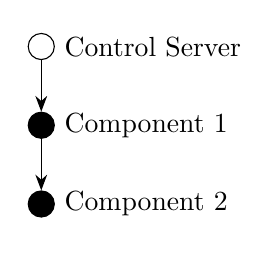
\begin{tikzpicture}[component/.style={draw,circle,fill}]
      \node[draw,circle,label=right:{Control Server}] at (0, 0) (controlServer) {};
      \node[component,label=right:{Component 1}] at (0, -1) (component1) {};
      \node[component,label=right:{Component 2}] at (0, -2) (component2) {};
      \draw[-{Stealth[length=2mm]}] (controlServer) -- (component1);
      \draw[-{Stealth[length=2mm]}] (component1) -- (component2);
    \end{tikzpicture}
    \caption{the topological structure of Figure~\ref{fig:components}}
    \label{fig:before_topology}
  \end{subfigure}
  \begin{subfigure}[b]{0.49\textwidth}
    \centering
    \begin{CenteredBox}
\begin{lstlisting}[escapechar=!]
- parents:
    - 0
  !\textcolor{verydarkgray}{<...>}!
- parents:
    - 0
  !\textcolor{verydarkgray}{<...>}!
- parents:
    - 1
    - 2
  !\textcolor{verydarkgray}{<...>}!
\end{lstlisting}
      \end{CenteredBox}
    \caption{changes necessary to define more complex topology}
    \label{fig:topology_implementation}
  \end{subfigure}
  \begin{subfigure}[b]{0.49\textwidth}
    \centering
    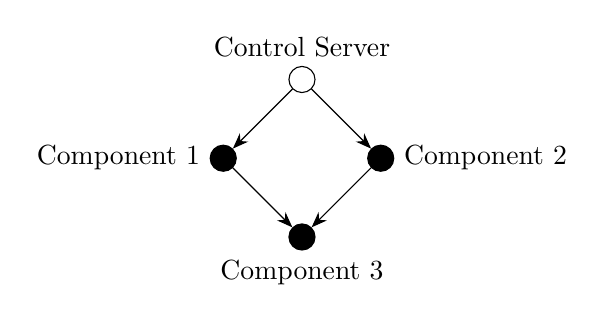
\begin{tikzpicture}[component/.style={draw, circle, fill}]
      \node[draw,circle,label=above:{Control Server}] at (0, 0) (controlServer) {};
      \node[component,label=left:{Component 1}] at (-1, -1) (component1) {};
      \node[component,label=right:{Component 2}] at (1, -1) (component2) {};
      \node[component,label=below:{Component 3}] at (0, -2) (component3) {};
      \draw[-{Stealth[length=2mm]}] (controlServer) -- (component1);
      \draw[-{Stealth[length=2mm]}] (controlServer) -- (component2);
      \draw[-{Stealth[length=2mm]}] (component1) -- (component3);
      \draw[-{Stealth[length=2mm]}] (component2) -- (component3);
    \end{tikzpicture}
    \caption{the topological structure of
      Figure~\ref{fig:topology_implementation}}
    \label{fig:after_topology}
  \end{subfigure}
  \caption{Component configuration files and their induced topologies}
\end{figure}

\subsection{What Happens During Execution} \label{sec:execution}

We illustrate some aspects of the execution and how different components
communicate with each other in Figure~\ref{fig:communication}. A sequence of
experiments begins with the initialisation of the start pod. At the start of
each experiment, the Flink app inside the start pod (called Benchmarker)
establishes the control server as a \texttt{socketTextStream}, i.e., the initial
source of data. It then constructs the DAG of components as described in
\texttt{components.yaml}.

The control server periodically sends messages to Benchmarker (as defined in
\texttt{global.yaml}). Each component (mapper) does three things upon receiving
each message:
\begin{enumerate}
\item First, it allocates an array of bytes so that the total memory usage would
  be as close to \texttt{memoryUsage} as possible. The array size is calculated
  using a linear regression model established using experimental data (see
  Section~\ref{sec:adjustments}).
\item Then, it creates a \texttt{String} object taking up \SI[number-math-rm =
  \mathnormal, parse-numbers = false]{\texttt{outputSize}}{\kibi\byte} of
  memory. This string will be passed to the next component in the chain.
\item Finally, it spends the remaining time (until total execution time is
  exactly \texttt{cpuTime}) testing the Collatz conjecture \cite{collatz} one
  initial integer at a time.
\end{enumerate}

After all messages from the control server pass through every component,
Benchmarker connects to the control server, sending it the total running time
(as measured by \texttt{JobExecutionResult.getNetRuntime()}). This number is
then rounded up to an integer number of minutes and used to retrieve performance
data for the time interval when the application was running.

Finally, for each metric defined in the global configuration file, the control
server establishes a connection to Prometheus, collects JSON data
recording the values of that metric in the last few minutes (as calculated
previously), and writes the data to a file (separate for each metric and
experiment) on the persistent volume. The files can then be transported to a
local directory by using MiniShift\footnote{Due to technical issues, an
  alternative to this step was not developed for deployment on OpenShift
  clusters.} SSH to copy them over to MiniShift host folder, which places them
into a local directory on the host machine. A Python script was written to
automate deploying the system, waiting for the control server to terminate, and
moving the files as described.

\begin{figure}
  \centering
  \begin{tikzpicture}
    \begin{umlseqdiag}
      \umlobject[no ddots]{Benchmarker}
      \umlobject[no ddots]{ControlServer}
      \umlobject[no ddots]{Prometheus}
      \umldatabase[no ddots]{PersistentVolume}
      \begin{umlfragment}[type=loop, label={$\forall$ experiments}, inner ysep=2]
        \umlsdnode[dt=3]{Benchmarker}
        \begin{umlcall}[op={initialise stream}]{Benchmarker}{ControlServer}
          \begin{umlfragment}[type=loop, label={$\forall$ messages}, inner xsep=7]
            \begin{umlcall}[op={message}, type=return]{ControlServer}{Benchmarker}
            \end{umlcall}
          \end{umlfragment}
        \end{umlcall}
        \begin{umlcall}[op={runtime}, type=return]{Benchmarker}{ControlServer}
        \end{umlcall}
        \begin{umlfragment}[type=loop, label={$\forall$ metrics}, inner xsep=6]
          \begin{umlcall}[op={query}, return={metric}]{ControlServer}{Prometheus}
          \end{umlcall}
          \begin{umlcall}[op={metric}]{ControlServer}{PersistentVolume}
          \end{umlcall}
        \end{umlfragment}
      \end{umlfragment}
    \end{umlseqdiag}
  \end{tikzpicture}
  \caption{Communication between different parts of the system visualised as a
    UML sequence diagram}
  \label{fig:communication}
\end{figure}

\section{Local Performance Tuning} \label{sec:adjustments}

The component class, responsible for using predefined amounts of resources, was
tested and adjusted locally, ensuring that it uses 100\% of a single CPU and
\SI[number-math-rm = \mathnormal, parse-numbers =
false]{\texttt{memoryUsage}}{\mebi\byte} of memory. Total heap usage was
measured for array sizes $2^0, 2^1, 2^2, \dots, 2^9$ and output strings of $2^0,
2^1, 2^2, \dots, \min \{ 2^8, \text{array size} \}$ characters (the output
string is constructed using the array, so the array size must always be at least
as big as the output string). Maximum heap usage was measured using GNU
Time\footnote{\url{https://www.gnu.org/software/time/}} and its Maximum Resident
Set Size metric. Each experiment was repeated three times, and median values
were taken.

We seek to know the average amount of memory used by a single character of a
Java string. Knowing that a single element of a byte array takes up exactly one
byte\footnote{This assumption was empirically confirmed in later experiments.}
allows us to reformulate the problem to a simple linear regression shown in
Figure~\ref{fig:regression1}. The model shows that overall memory usage can be
expressed as
\begin{equation} \label{eq:regression}
  \text{memory usage} = \SI{40}{\mebi\byte} + \text{array size} + 3.268 \times
  \text{string size} + \epsilon,
\end{equation}
contradicting the common wisdom that a character uses approximately two bytes of
memory \cite{java_memory}.

Figure~\ref{fig:regression2} presents a more detailed view, but suggests
the same conclusion. While the predictions seem to consistently overestimate
memory consumption for short strings and similarly underestimate it for longer
strings, adding a quadratic term is not enough to remove the bias in errors, and
the errors are sufficiently small.

\begin{figure}
  \centering
  \begin{minipage}{.49\textwidth}
    \centering
    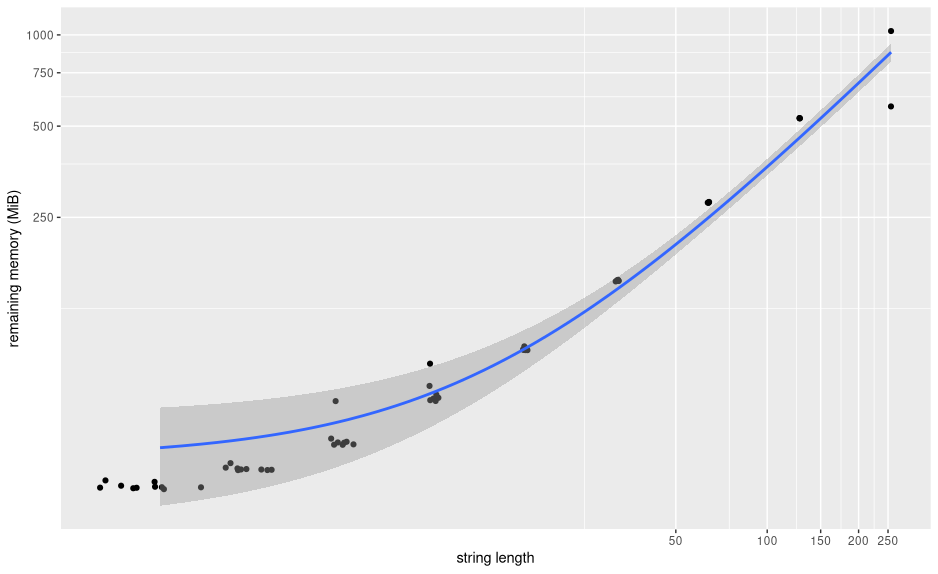
\includegraphics[width=\linewidth]{../local_experiments/memory_tests/prediction2.png}
    \captionof{figure}{A log-log plot comparing the number of characters in a string and the
      observed memory unaccounted by the array. In each column, separate points
      correspond to different array sizes (plotted with jitter). The blue curve is a
      best-fit linear regression line, and the shaded area marks one standard
      error.}
    \label{fig:regression1}
  \end{minipage}\hfill%
  \begin{minipage}{.49\textwidth}
    \centering
    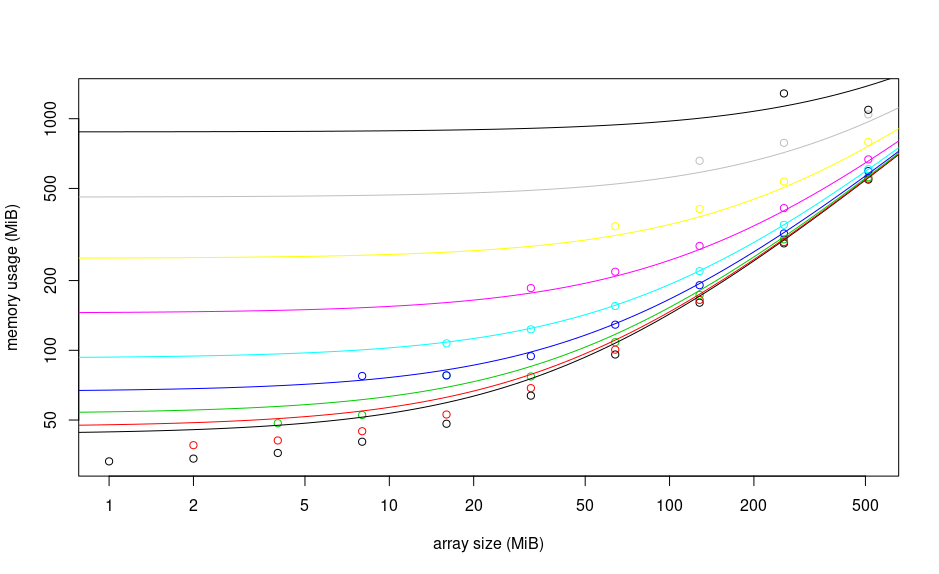
\includegraphics[width=\textwidth]{../local_experiments/memory_tests/prediction1.png}
    \captionof{figure}{A log-log plot showing memory consumption across a range of array
      sizes, with different string sizes represented by different colours. For
      each string size, we also draw a regression line in the corresponding
      colour.}
    \label{fig:regression2}
  \end{minipage}
\end{figure}

\paragraph{Adjusted Performance}

We can use the two numerical parameters in Equation~\eqref{eq:regression} to
adjust our component class in order to ensure that it uses the right amount
of memory. We run a similar set of experiments as before, except replacing array
size with expected memory usage as one of our independent variables (the other
being string size). Memory usage is set to four different values: 64, 128,
256, and \SI{512}{\mebi\byte} (note that the smallest possible memory usage is
about \SI{40}{\mebi\byte}), while string size is exponentially increased from
\SI{1}{\mebi\byte} up to the largest power of two small enough so that the
string can be constructed from the array. We plot the errors in
Figure~\ref{fig:adjustment}. Note that the largest error is smaller than
\SI{50}{\kibi\byte}, which is good enough for our needs.

\begin{figure}
  \centering
  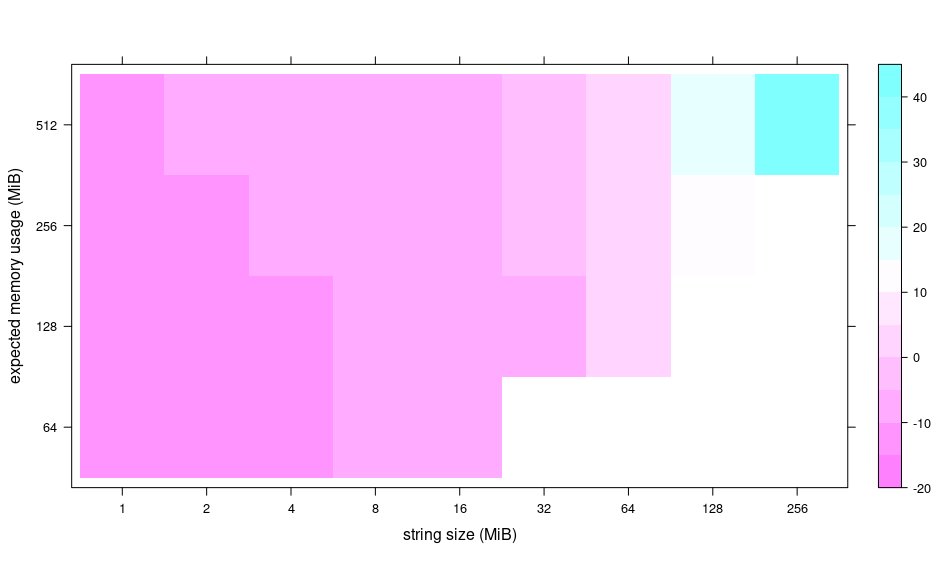
\includegraphics[width=0.5\textwidth]{../local_experiments/memory_tests/adjusted.png}
  \caption{A heat map of errors (in \si{\kibi\byte})}
  \label{fig:adjustment}
\end{figure}

\section{Experimental Evaluation} \label{sec:experiments}

Experiments were performed in order to determine how well performance metrics
observed with a standalone Java application transfer to MiniShift. We explore
four values of \texttt{memoryUsage} (\SI{64}{\mebi\byte}, \SI{128}{\mebi\byte},
\SI{256}{\mebi\byte}, \SI{512}{\mebi\byte}), while keeping \texttt{cpuTime} at
zero so that each run lasts only as long as it takes to allocate and randomise
the memory. For \texttt{outputSize}, we explore every power-of-two number of
\si{\mebi\byte} compatible with the current \texttt{memoryUsage} value. We stick
to a single component and record CPU and memory consumption at \SI{1}{\second}
intervals using Prometheus. Each \texttt{memoryUsage} and \texttt{outputSize}
configuration is written into \texttt{components.yaml} and run three times. With
each run, we recreate all OpenShift components (pods, services, etc.), wait for
the start pod to terminate, and retrieve the generated JSON files.

Figure~\ref{fig:cpu_experiment} shows CPU usage across all runs. Even
though our standalone Java application easily reaches 100\% CPU usage, when
transferred to an OpenShift environment, a typical run could only get around
10\%--15\% (as indicated by the red curve), occasionally reaching up to 70\% or
80\% CPU usage. This can be explained by the fact that MiniShift internal
processes as well as Flink JobManager and TaskManager are all running on the
same machine. Even though the processes are distributed among eight cores, this
overhead is sufficient to significantly decelerate the application.

\begin{figure}
  \centering
  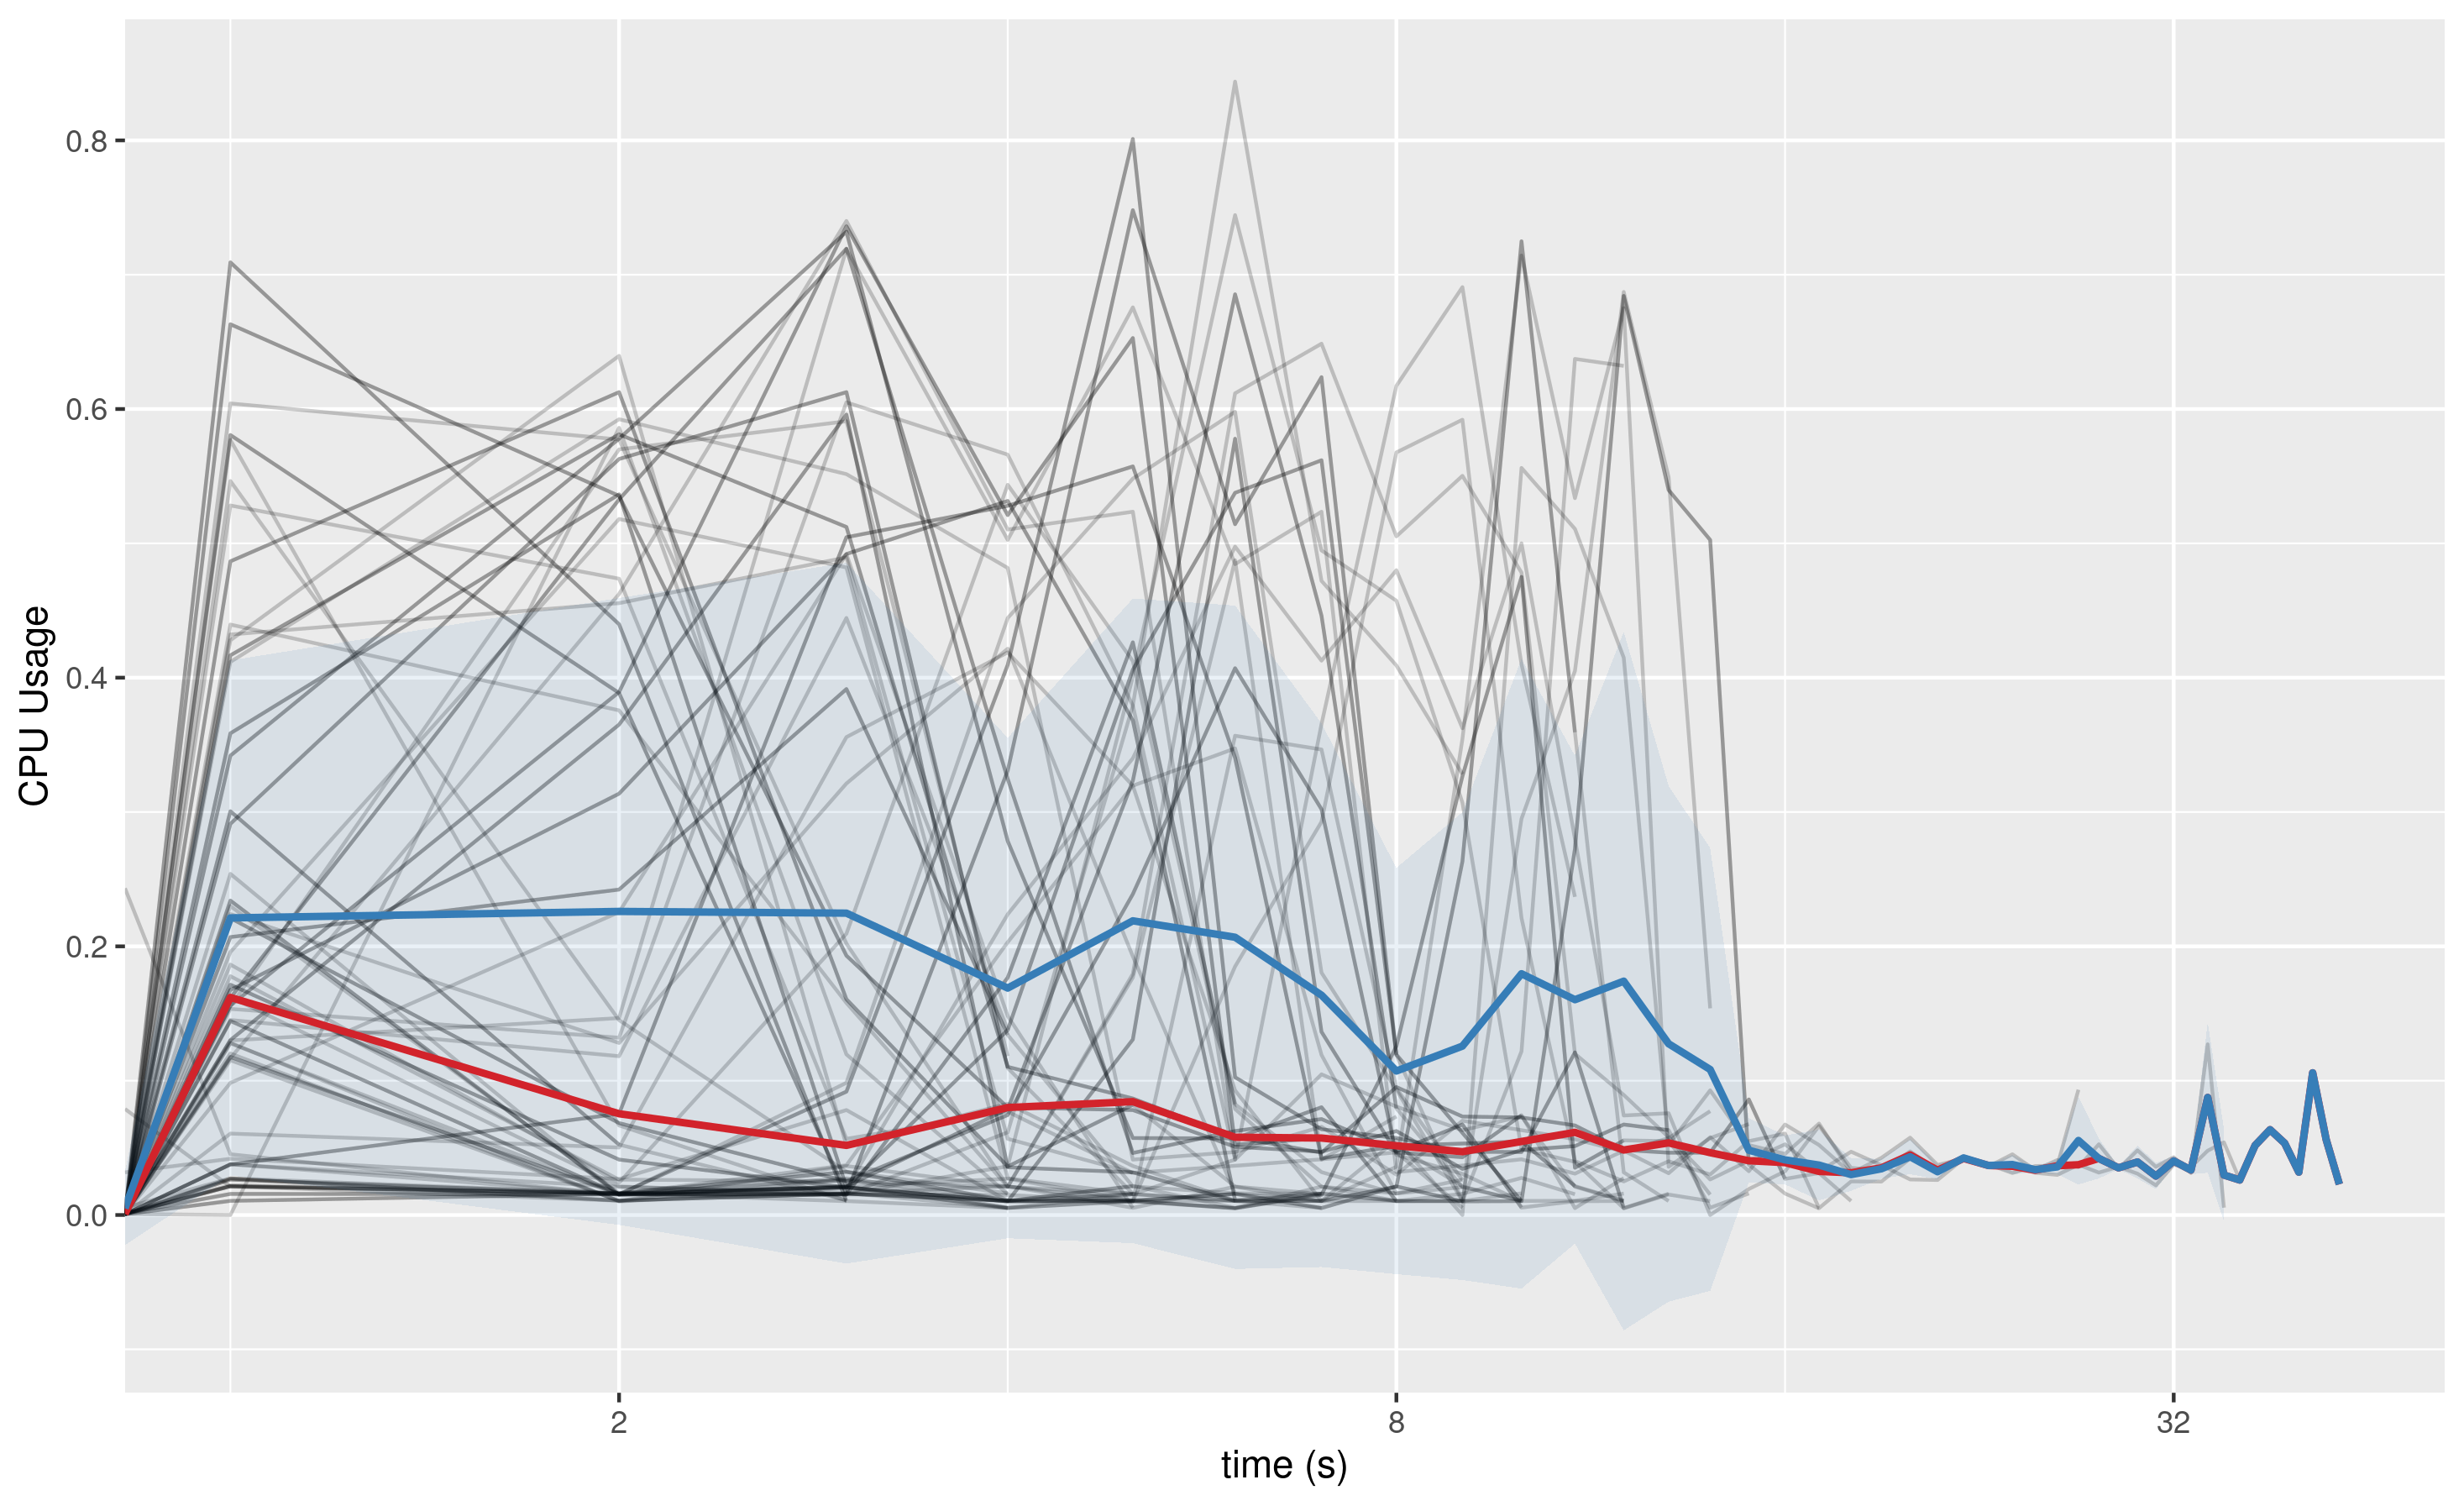
\includegraphics[width=\textwidth]{../plots/cpu_experiment.png}
  \caption{CPU usage across time. Each gray line represents a different run. The
  red curve is their (pointwise) median, the blue curve is the mean, while the
  shaded area marks one standard deviation around the mean. Note that time is on a
  $\log$ scale.}
  \label{fig:cpu_experiment}
\end{figure}

Figure~\ref{fig:heap_experiment} shows similar memory usage measurements divided
into four plots, one for each value of \texttt{memoryUsage}. We can see that
there is significant variation among runs (and different \texttt{outputSize}
values). In fact, in order to determine whether memory usage is optimal or
hampered, one would need to run many identical experiments to account for
variability. Moreover, each curve is unlikely to be fully summarised by a single
number: maximum values are almost always higher than the expected result, while
means are likely to be distorted by the initial several seconds of low memory
usage as well as observed dips in memory usage later in the execution.

Note that each individual run can be summarised as follows:
\begin{enumerate}
\item Memory usage starts low.
\item It rises two times.
\item Sometimes memory usage experiences a significant drop, and sometimes this
  step is skipped.
\item Memory usage stays constant for a while.
\item The process terminates.
\end{enumerate}
We can easily explain this pattern. The first increase is caused by the array
allocation, while the second one is the result of constructing the output
string. The drop in memory usage happens when the array is deallocated
(garbage-collected) some time after the execution of my code completes.
Sometimes that happens early enough to be captured by Prometheus, and sometimes
the Flink job is marked as complete before garbage collection activates.

\begin{figure}
  \centering
  \begin{subfigure}[t]{0.49\textwidth}
    \centering
    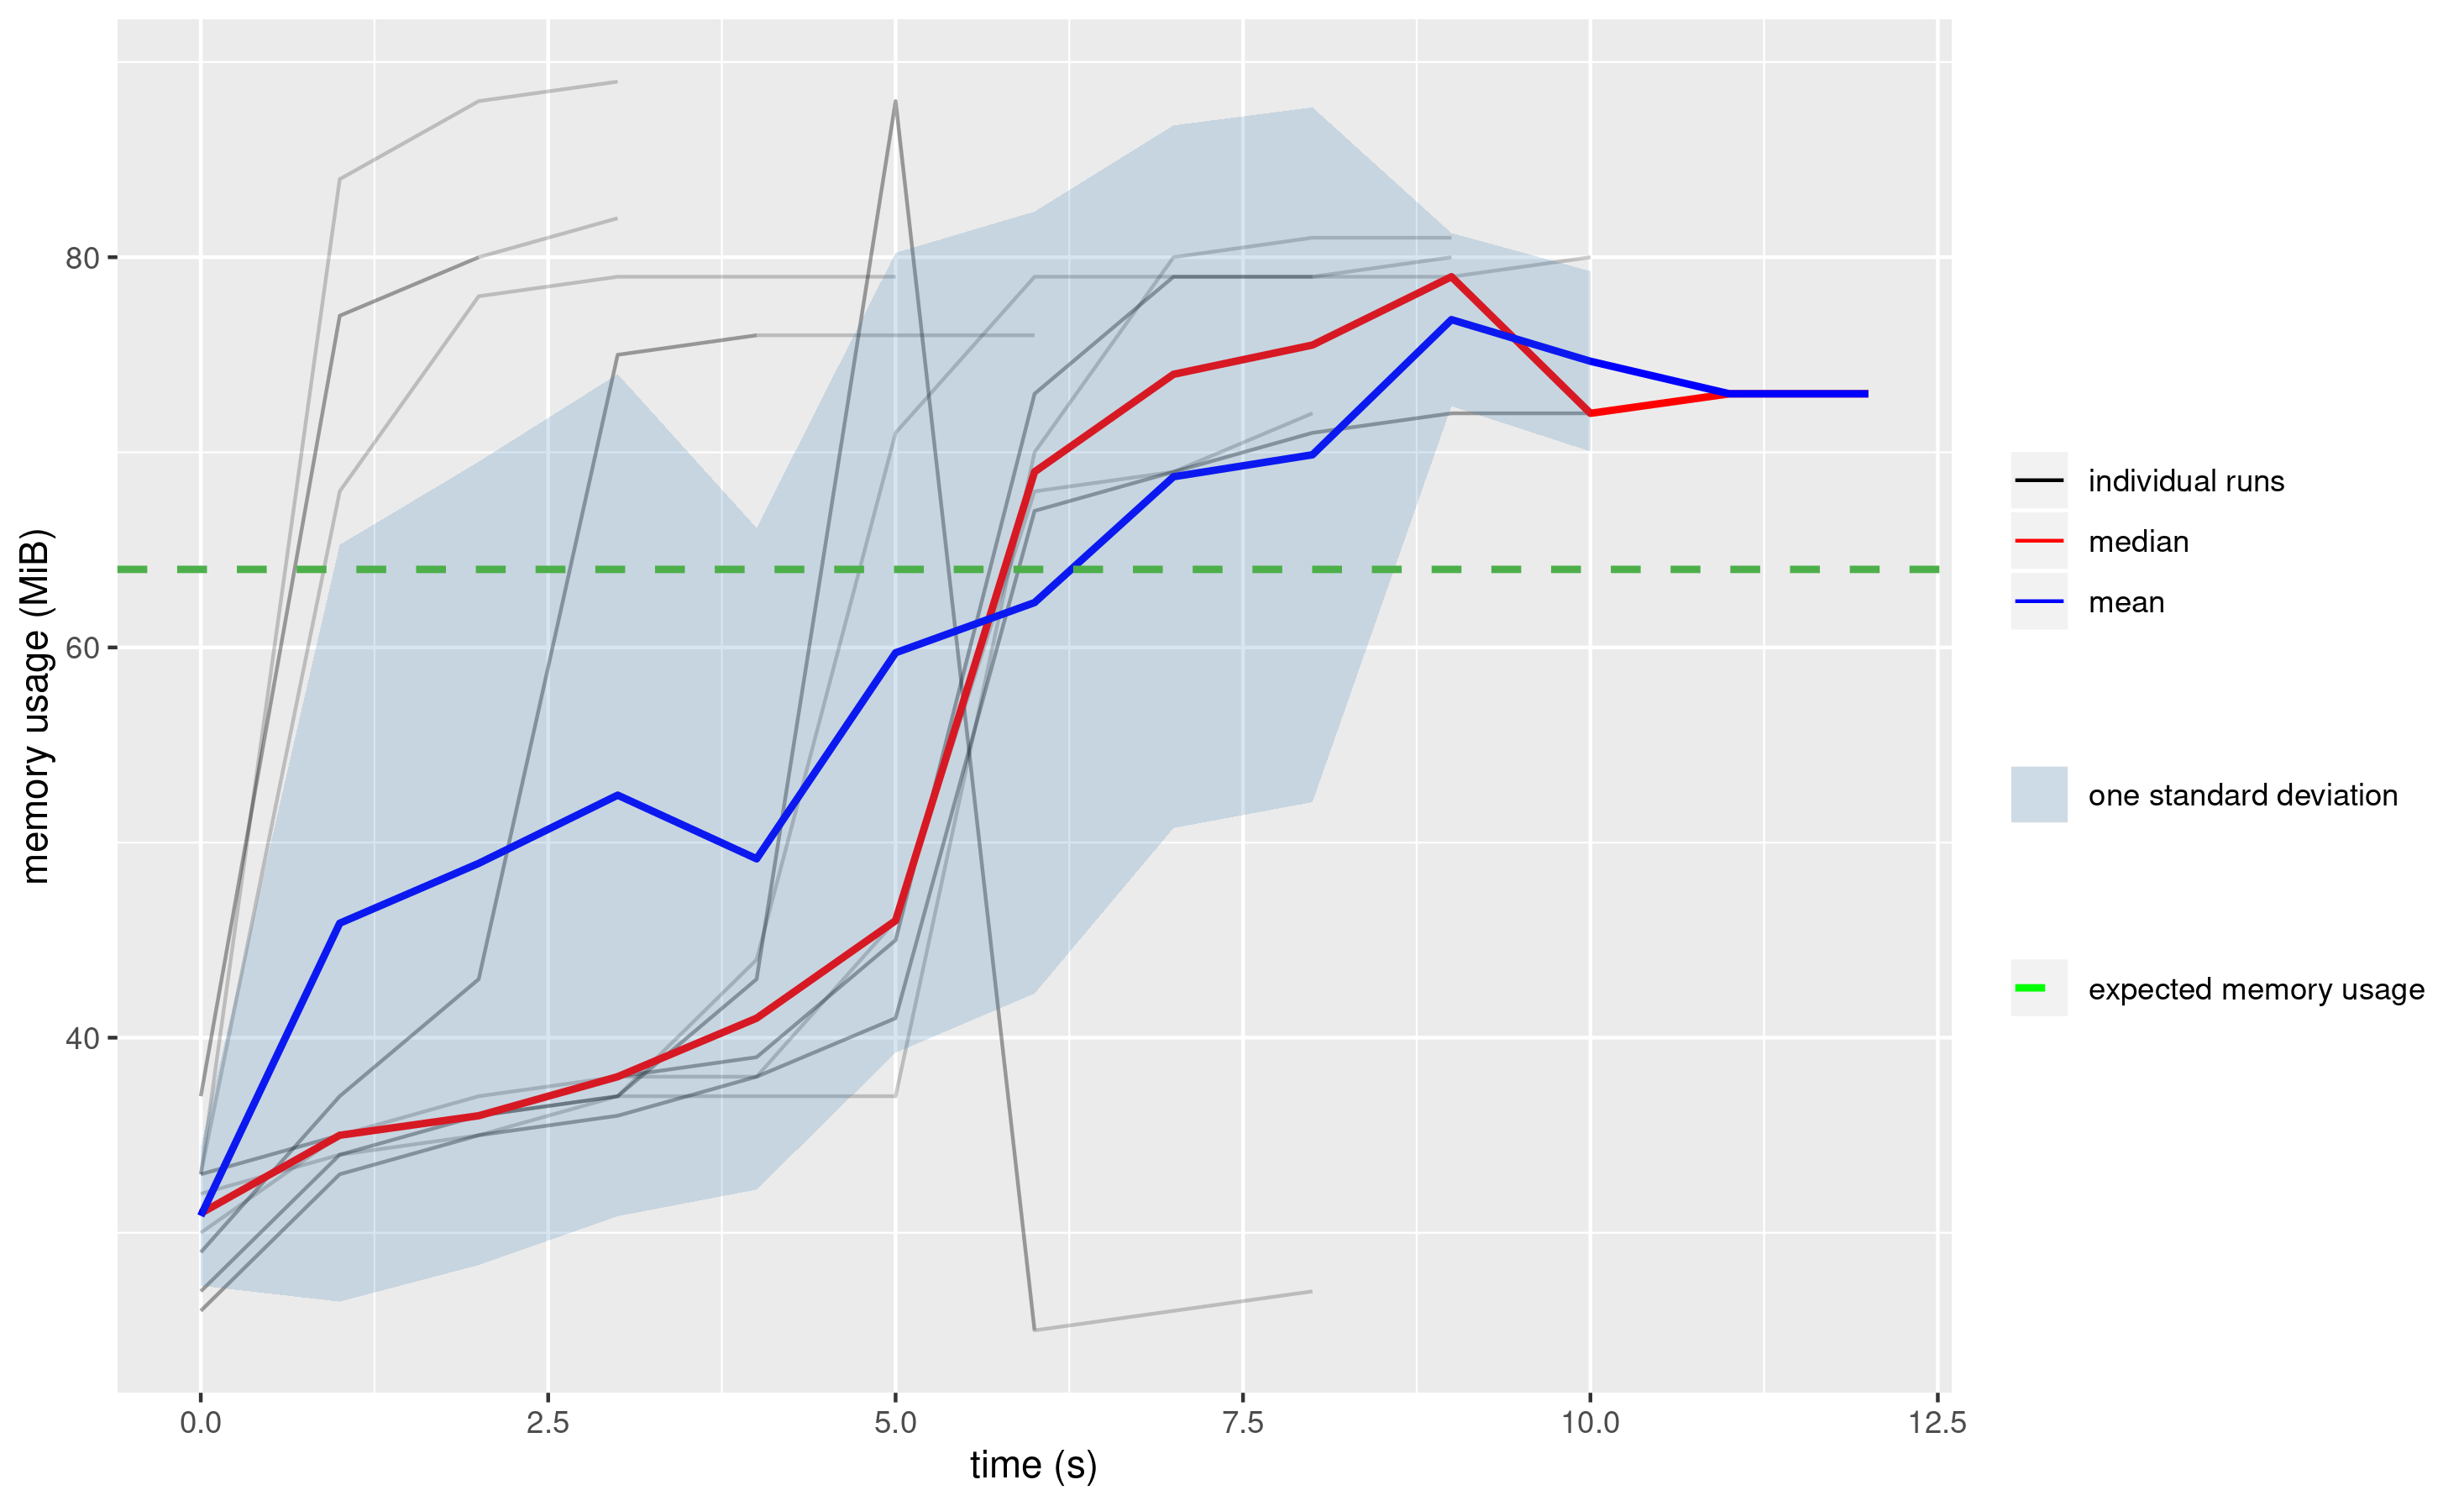
\includegraphics[width=\textwidth]{../plots/heap_64.png}
    \caption{expected heap usage: \SI{64}{\mebi\byte}}
    \label{fig:heap_64}
  \end{subfigure}
  \begin{subfigure}[t]{0.49\textwidth}
    \centering
    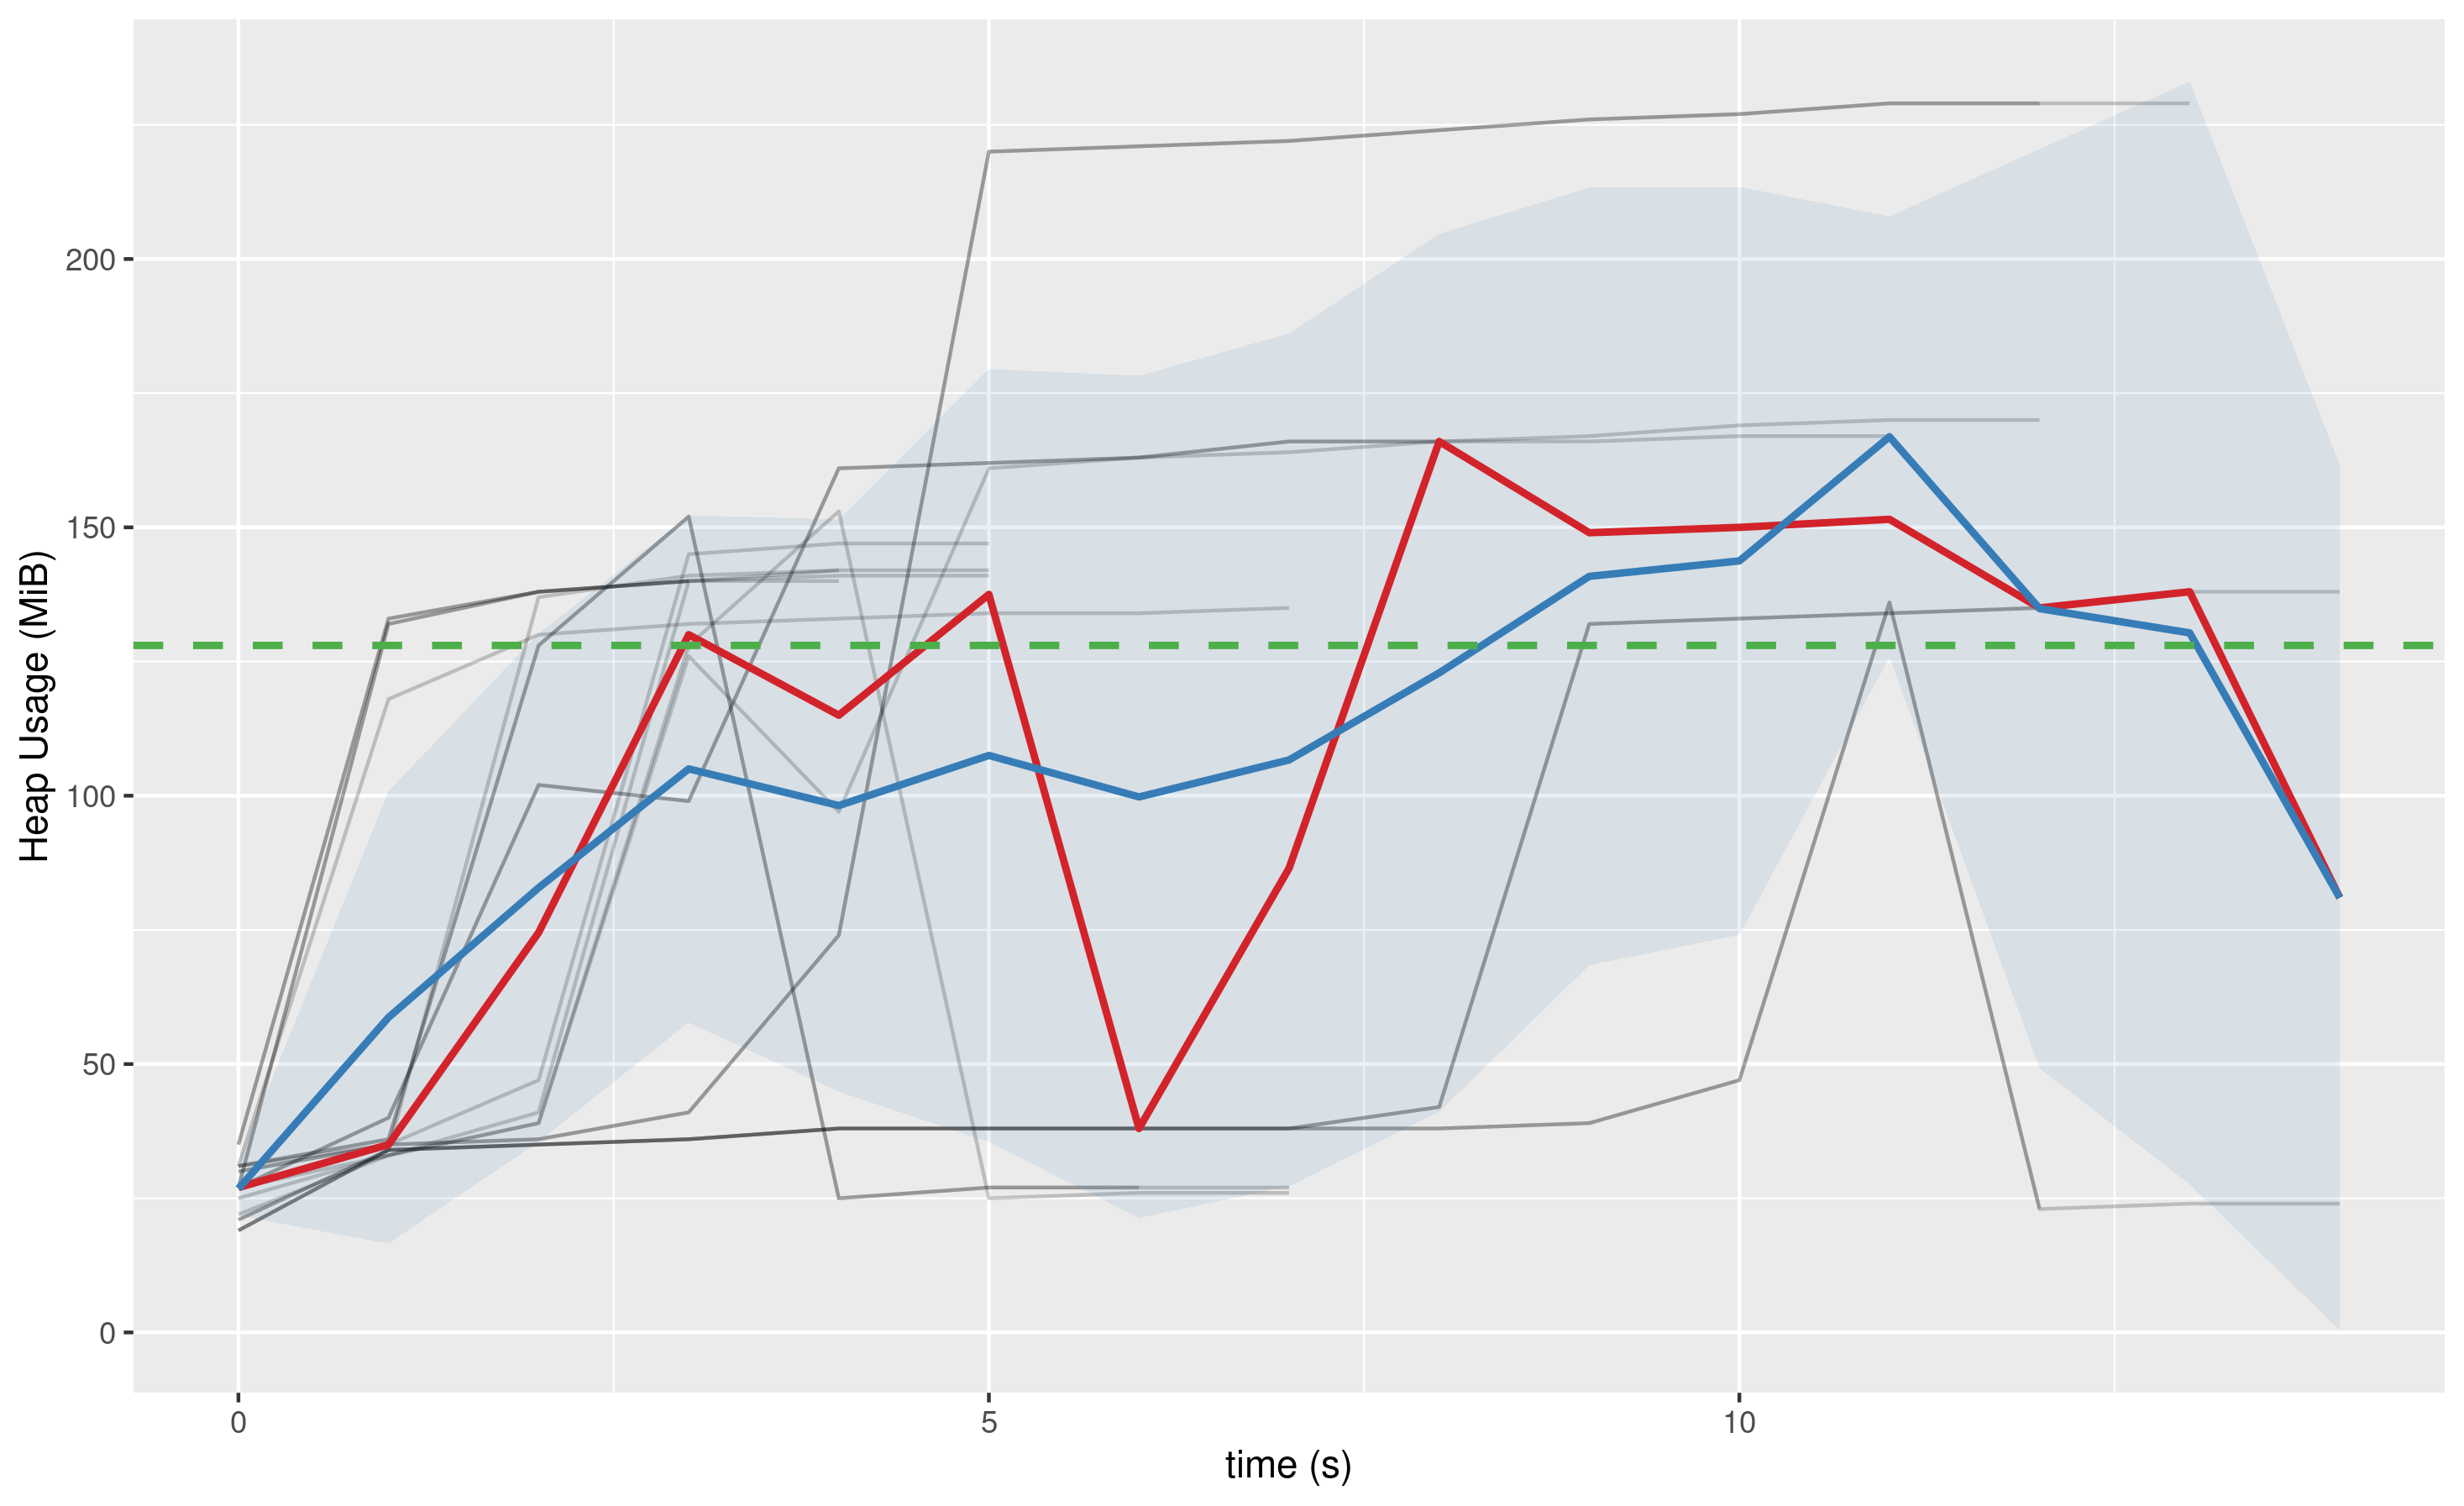
\includegraphics[width=\textwidth]{../plots/heap_128.png}
    \caption{expected heap usage: \SI{128}{\mebi\byte}}
    \label{fig:heap_128}
  \end{subfigure}
  \begin{subfigure}[t]{0.49\textwidth}
    \centering
    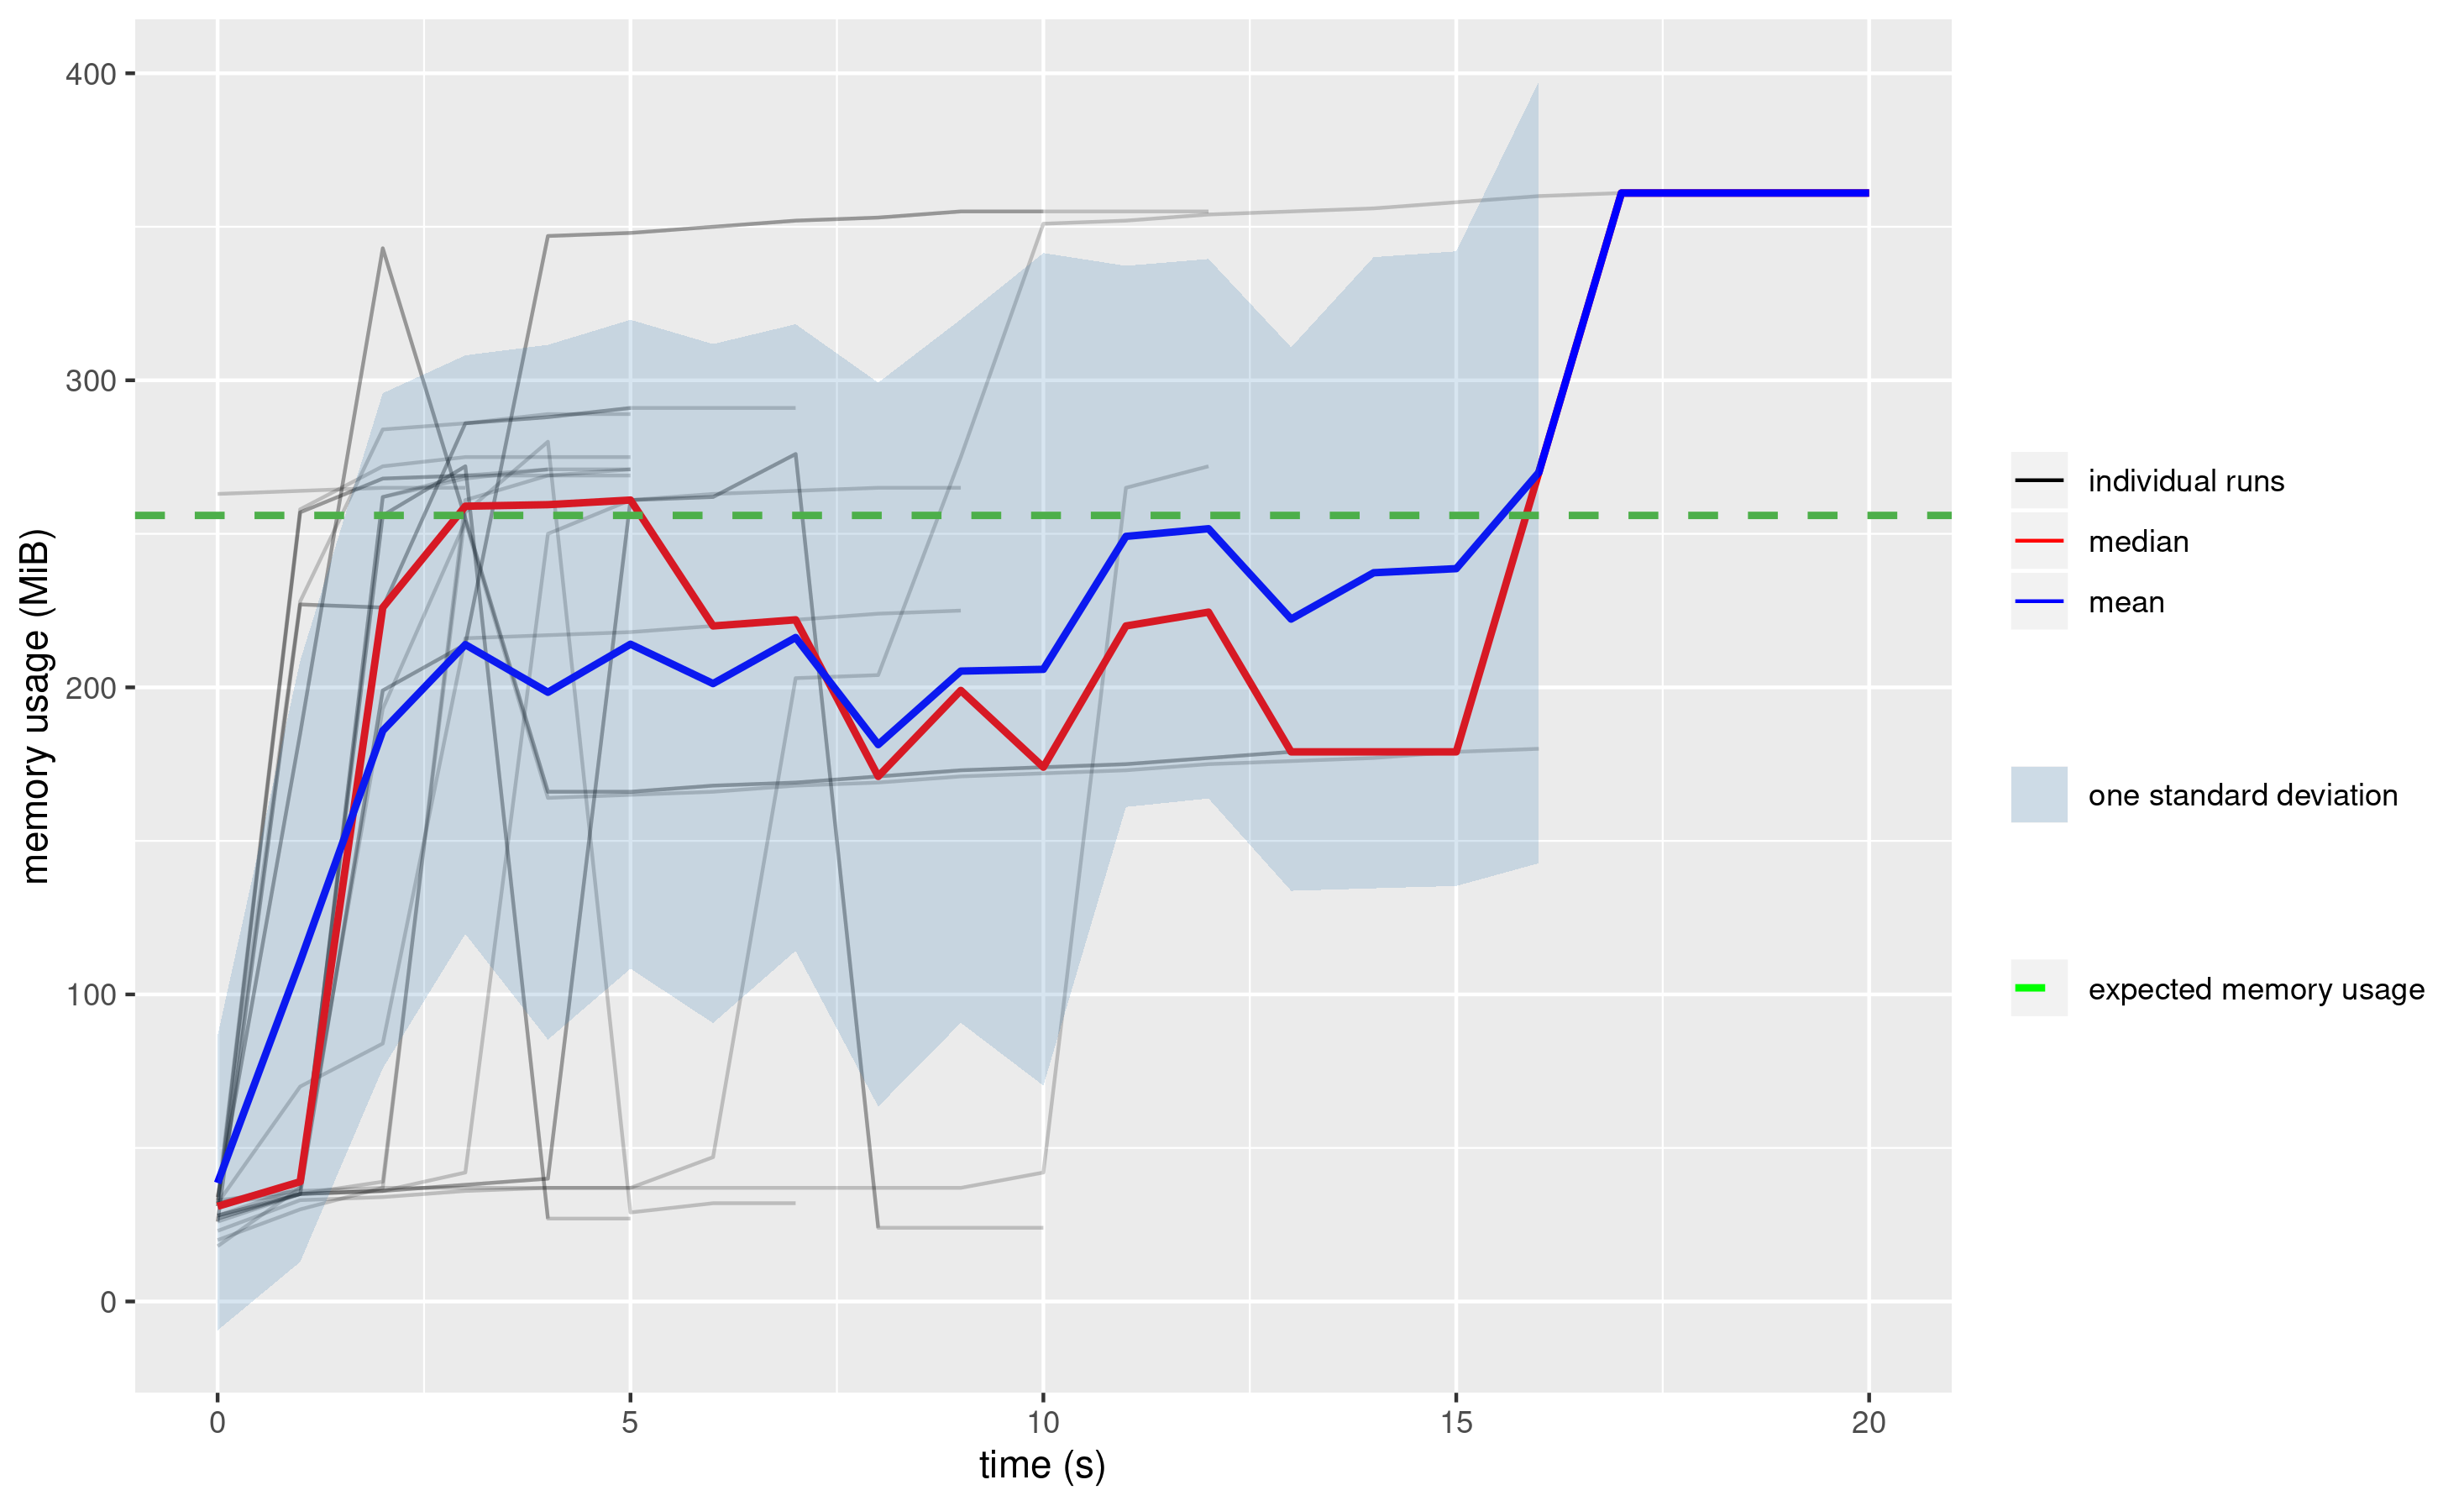
\includegraphics[width=\textwidth]{../plots/heap_256.png}
    \caption{expected heap usage: \SI{256}{\mebi\byte}}
    \label{fig:heap_256}
  \end{subfigure}
  \begin{subfigure}[t]{0.49\textwidth}
    \centering
    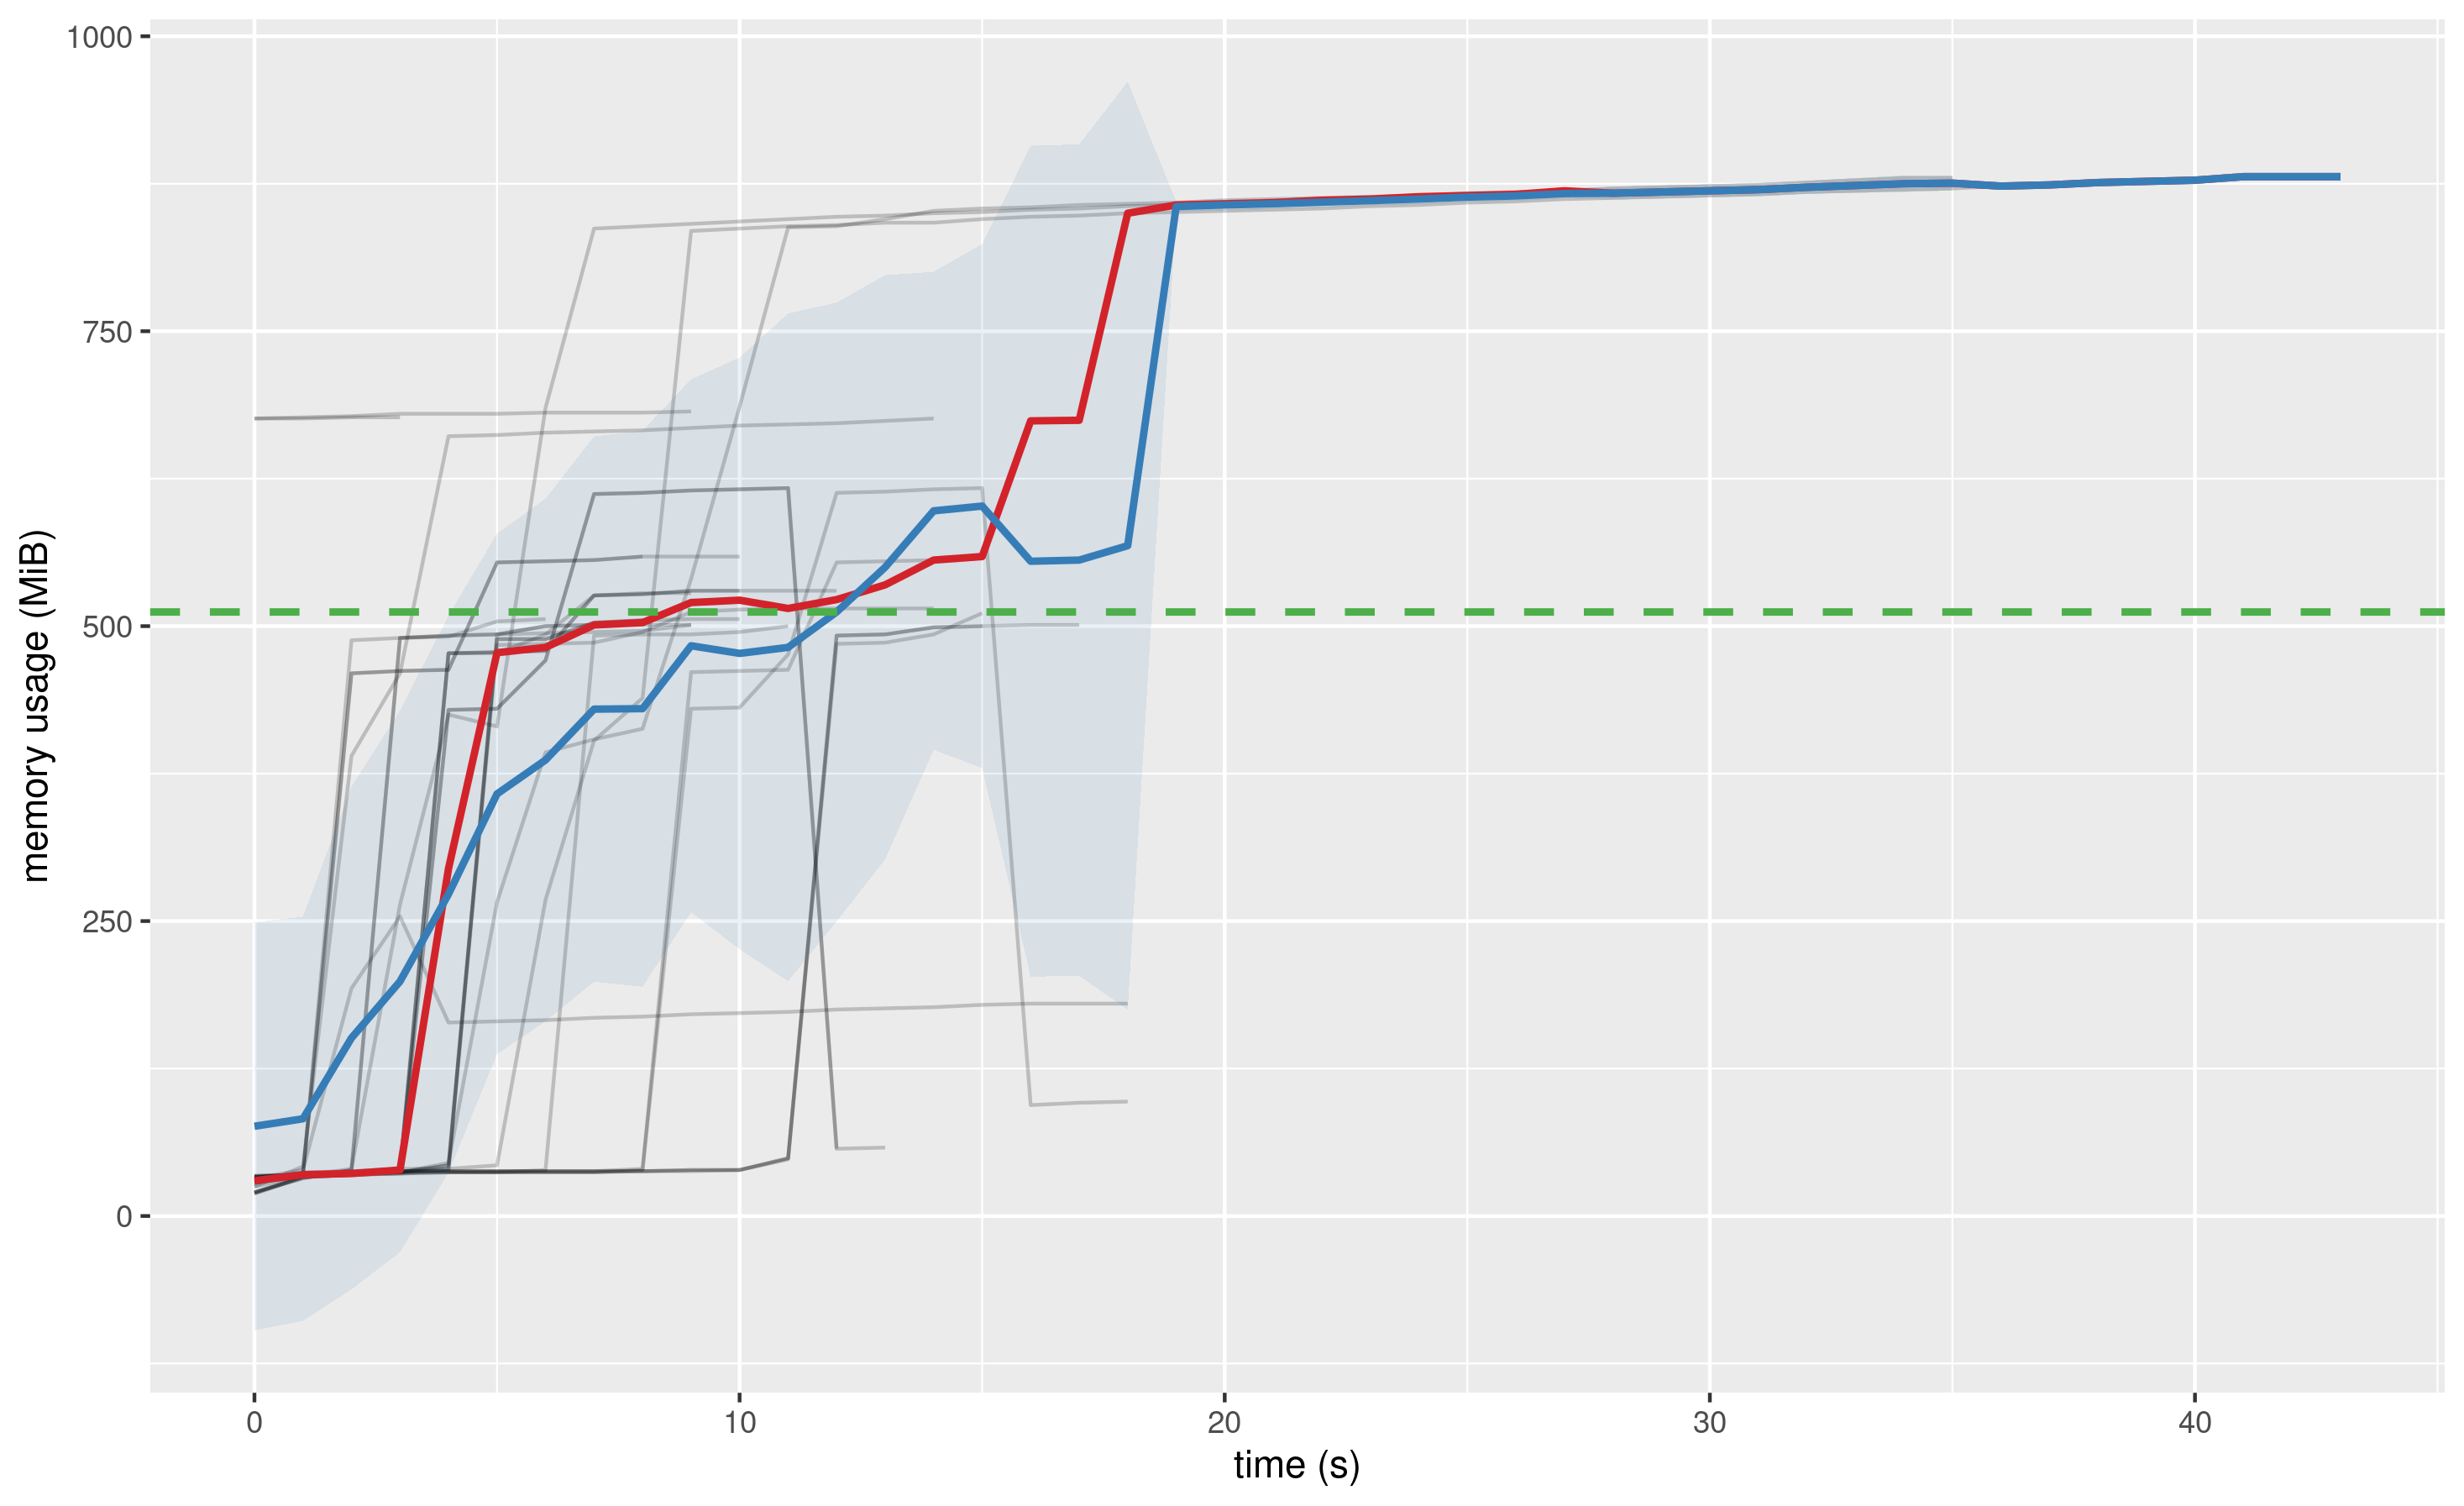
\includegraphics[width=\textwidth]{../plots/heap_512.png}
    \caption{expected heap usage: \SI{512}{\mebi\byte}}
    \label{fig:heap_512}
  \end{subfigure}
  \caption{Observed versus expected memory usage across time for four expected
    memory amounts. The green dashed horizontal line marks the expected amount
    of memory usage. Each gray line represents a different run. The red curve is
    their (pointwise) median, the blue curve is the mean, while the shaded area
    marks one standard deviation around the mean.}
  \label{fig:heap_experiment}
\end{figure}

Finally, we consider the extent to which memory usage can be summarised by
taking the maximum across time. We report each difference between expected $E$
and observed $O$ values as a relative error, i.e.,
\[
  \frac{O - E}{E}.
\]
We consider these errors for all viable combinations of \texttt{memoryUsage} and
\texttt{outputSize} and report the median of the three identical runs performed
on each combination. The results are in Figure~\ref{fig:relative_errors}.
Unsurprisingly, maximum memory usage across time is usually higher than the
estimate. Also note that the overall shape of the heat map is similar to
Figure~\ref{fig:adjustment}, where we measure differences between observed and
expected memory usage with the standalone Java application. In both cases,
observed values are smaller with lower values of \texttt{outputSize}, and a
combination of high overall memory usage and a long output string in the top
right corner of both heat maps is likely to result in observed memory usage
being significantly higher than the expected value. Even though we take median
values to reduce the effect of outliers, observed memory usage can be up to 80\%
higher than the expected value, adding evidence to the imprecision and
unreliability of making judgments based on a single number or a single
experiment.

\begin{figure}
  \centering
  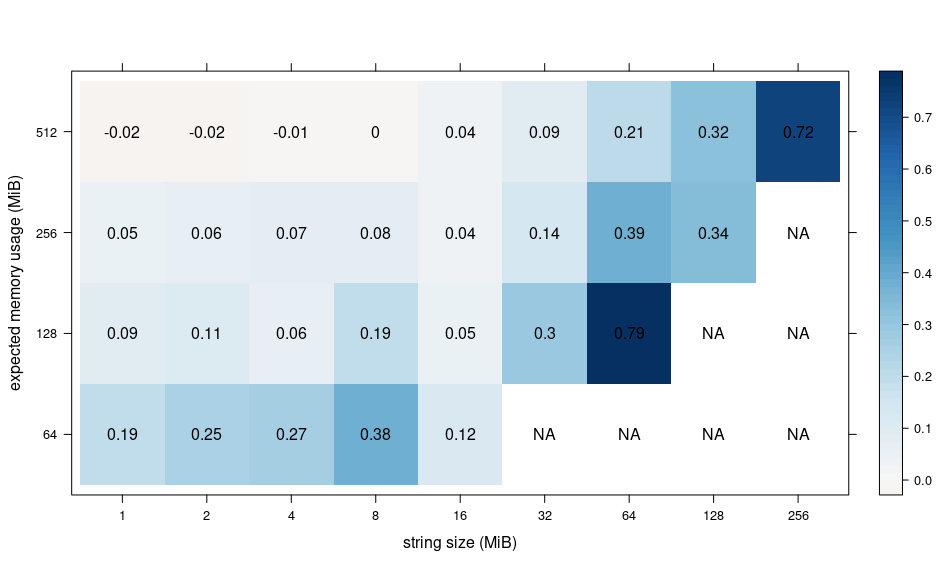
\includegraphics[width=0.5\textwidth]{../plots/relative_median_errors.png}
  \caption{Relative median memory usage errors, as predicted by the maximum
    memory usage across execution}
  \label{fig:relative_errors}
\end{figure}

\section{Example Applications} \label{sec:example_applications}

\paragraph{A Simple Website}

\begin{table}
  \centering
  \caption{Performance statistics of the top 100 e-commerce websites}
  \begin{tabular}{l c c c}
    \toprule
    Metric & min & mean & max \\
    \midrule
    Page load time (\si{\second}) & \tablenum{0.468} & \tablenum{2.67} & \tablenum{9.67} \\
    Page size (\si{\mebi\byte}) & \tablenum{0.719} & \tablenum{3.03} & \tablenum{14.21} \\
    Number of requests made per load & \num{45} & \num{192} & \num{660} \\
    \bottomrule
  \end{tabular}
  \label{tbl:web}
\end{table}

In order to simulate a website, we need some data about the performance metrics
of a typical website. We extract the data in Table~\ref{tbl:web} from
experiments run on popular websites \cite{web_performance}. Thus, we can
simulate an average website with a single component by making the following
modelling assumptions:
\begin{itemize}
\item $\texttt{cpuTime} = \frac{\text{page load time}}{\text{number of requests
      per load}} = \frac{\SI{2.67}{\second}}{192} \approx \SI{0.014}{\second}$;
\item \texttt{memoryUsage} is minimal, i.e., the smallest amount necessary to
  construct the output string;
\item $\texttt{outputSize} = \frac{\text{page size}}{\text{number of requests
      per load}} = \frac{\SI{3.03}{\mebi\byte}}{192} = \SI{16.16}{\kibi\byte}$;
\item $\texttt{messagesPerBatch} = \text{number of requests per load} = 192$.
\end{itemize}

\paragraph{A Machine Learning System}

For a realistic model of a machine learning (ML) system, we measured a
classification system used to construct algorithm portfolios (akin to
\cite{DBLP:conf/lion/KotthoffMS16}) implemented using an R package
\texttt{llama} \cite{kotthoff_llama_2013} and run on a thousand maximum common
subgraph problems and three algorithms. The resulting performance metrics are
displayed in Figure~\ref{fig:ml_diagram}, with each component's
\texttt{outputSize} positioned next to its outgoing arrow. Sending a single
message, then, corresponds to selecting a subset of data, generating features,
and training an ML model. Note that the last two parameters define each
component's I/O (i.e., file-reading) properties and can be easily ignored
(otherwise see Section~\ref{sec:io}). Other I/O-related parameters are assumed
to be big enough (or small enough) so that their exact values are irrelevant to
the performance of the system.

\setlength{\tabcolsep}{3pt}
\begin{figure}
  \centering
  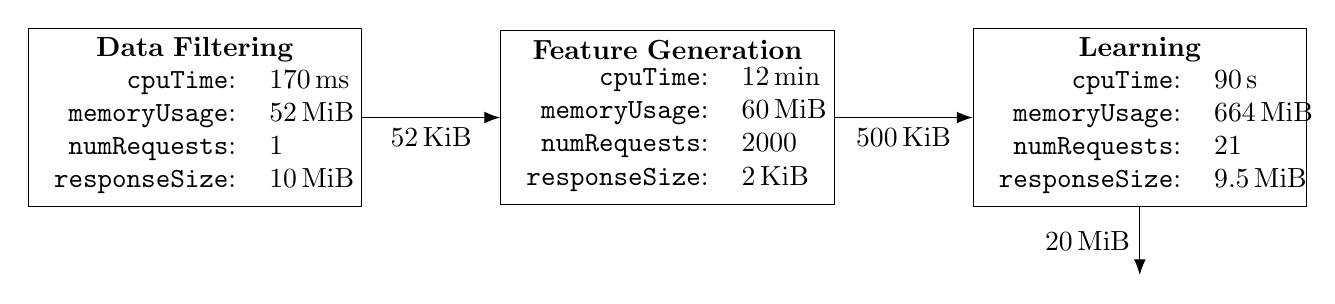
\begin{tikzpicture}[component/.style={draw, text width=4cm, align=center}]
    \node[component] at (0, 0) (filtering) {
      \textbf{Data Filtering}\\
      \begin{tabular}{r l}
        \texttt{cpuTime}: & \SI{170}{\milli\second}\\
        \texttt{memoryUsage}: & \SI{52}{\mebi\byte}\\
        \texttt{numRequests}: & \num{1}\\
        \texttt{responseSize}: & \SI{10}{\mebi\byte}
      \end{tabular}
    };
    \node[component] at (6, 0) (features) {
      \textbf{Feature Generation}\\
      \begin{tabular}{r l}
        \texttt{cpuTime}: & \SI{12}{\minute}\\
        \texttt{memoryUsage}: & \SI{60}{\mebi\byte}\\
        \texttt{numRequests}: & \num{2000}\\
        \texttt{responseSize}: & \SI{2}{\kibi\byte}
      \end{tabular}
    };
    \node[component] at (12, 0) (learning) {
      \textbf{Learning}
      \begin{tabular}{r l}
        \texttt{cpuTime}: & \SI{90}{\second}\\
        \texttt{memoryUsage}: & \SI{664}{\mebi\byte}\\
        \texttt{numRequests}: & \num{21}\\
        \texttt{responseSize}: & \SI{9.5}{\mebi\byte}
      \end{tabular}
    };
    \draw[-{Latex[length=2mm]}] (filtering) -- node[below] {\SI{52}{\kibi\byte}} (features);
    \draw[-{Latex[length=2mm]}] (features) -- node[below] {\SI{500}{\kibi\byte}} (learning);
    \draw[-{Latex[length=2mm]}] (learning) -- node[left] {\SI{20}{\mebi\byte}} (12, -2);
  \end{tikzpicture}
  \caption{A model for a machine learning system, displaying typical resource
    usage metrics}
  \label{fig:ml_diagram}
\end{figure}
\setlength{\tabcolsep}{6pt}

\section{Input/Output Simulation} \label{sec:io}

I/O simulation is meant to simulate a gradual memory growth, as if querying a
database for relational data or downloading a large file. In order to add I/O
simulation to a model, one can simply add an optional \texttt{io} clause to the
description of a component in the \texttt{components.yaml} file, containing the
following parameters:
\begin{description}
\item[$\texttt{mode} \in \{ \text{startup}, \text{regular} \}$]
  determines when to simulate I/O: during the initialisation stage or with every
  call to \texttt{map()}.
\item[\texttt{numRequests}] is the number of request-response interactions
  between the component and the (simulated) data source.
\item[\texttt{responseSize}] is the size of the response (in \si{\kibi\byte}).
\item[\texttt{latency}] is the amount of time spent between a request
  and receiving the first byte of the response (in \si{\milli\second}).
\item[\texttt{bandwidth}] is the bandwidth for transferring the response (as the
  request is assumed to be small) (in
  \si[per-mode=symbol]{\mebi\bit\per\second}).
\item[\texttt{intervalBetweenRequests}] is the amount of time between receiving
  a response and sending another request (in \si{\milli\second}).
\end{description}
For example, Figure~\ref{listing:io} defines a component that receives its
input from the control server. For each message, it takes \SI{5}{\milli\second}
to execute, uses \SI{0}{\mebi\byte} of memory\footnote{Obviously, more memory
  and/or CPU time may be needed to satisfy other parts of the component's
  definition, in which case the declared numbers act like lower bounds.}, and
produces an output string of \SI{1}{\kibi\byte}. Furthermore, for each message,
it also performs an I/O simulation that consists of receiving two files of
\SI{2}{\kibi\byte} each at \SI[per-mode=symbol]{1000}{\mebi\byte\per\second}, where the
server `serving' the files has a latency of \SI{10}{\milli\second} and there is
a \SI{10}{\milli\second} delay between downloading the files. Note that the
top-level parameters such as \texttt{cpuTime} and \texttt{memoryUsage} take into
account the running time and memory usage of I/O simulations.

\begin{figure}
  \centering
  \begin{CenteredBox}
\begin{lstlisting}
- parents:
    - 0
  cpuTime: 5
  memoryUsage: 0
  outputSize: 1
  io:
    mode: regular
    numRequests: 2
    responseSize: 2
    latency: 10
    bandwidth: 1000
    intervalBetweenRequests: 10
\end{lstlisting}
  \end{CenteredBox}
  \caption{An example component with I/O simulation}
  \label{listing:io}
\end{figure}

We can then use these variables to simulate an I/O dialogue as described in
Algorithm~\ref{alg:io} (with unit conversion skipped for
simplicity). We use the variable $s$ to track our `sleep debt', i.e., the amount
of time the algorithm is supposed to sleep for at the end of each iteration on
line~\ref{alg:main_sleep}. The function \texttt{mySleep} was added in order to
ignore sleeping instructions for amounts of time smaller than
\SI{15}{\milli\second} because most commonly-used operating systems have no
support for this level of real-time behaviour control. We start by sleeping for
\SI[number-math-rm=\mathnormal,parse-numbers=false]{\texttt{latency}}{\milli\second}
to simulate the first delay between sending the request and receiving the data;
other \texttt{latency} delays are incorporated into $s$ on
line~\ref{alg:s_plus_latency}. For each request, we gradually build up a linked
list $L$ until it uses about
\SI[number-math-rm=\mathnormal,parse-numbers=false]{\texttt{responseSize}}{\kibi\byte}
memory. Setting the size of a single linked list node as \texttt{NODE\_SIZE}
allows us to calculate that we need
$\frac{\texttt{responseSize}}{\texttt{NODE\_SIZE}}$ nodes in order to use the
desired amount of memory (we round down in the algorithm). Similarly, in order
to achieve the right \texttt{bandwidth}, we need each node to be constructed in
$\frac{\texttt{NODE\_SIZE}}{\texttt{bandwidth}}$ time.

Based on separate experimental evidence, adding a single random integer to a
linked list typically takes about \SI{98}{\nano\second}. While this amount of
time is negligible for small lists, it can add up to significant delays when
considering linked lists with millions of nodes. To take this into account, we
measure the amount of time the yellow block of code takes to execute and
subtract it from $s$ on line~\ref{alg:subtract_time}. The yellow block is
supposed to take $\frac{\texttt{responseSize}}{\texttt{bandwidth}}$ time, so we
add the difference between the expectation and the reality to the amount of time
the algorithm sleeps at the end of each iteration. If this is not the final
iteration of the outer for loop, we also add \texttt{intervalbBetweenRequests}
and \texttt{latency} as well. The function of $s$ is to collect multiple
reasons to sleep into a single call to \texttt{mySleep} as well as to take into
account the amount of time it takes to build the linked list. If $s$ is negative
or too small, we let it influence the simulation of the next request so that the
total amount of time is as accurate as possible. Otherwise, we sleep for the
desired amount of time and reset $s$ back to zero.

\begin{algorithm}
  \SetKwData{numRequests}{numRequests}
  \SetKwData{latency}{latency}
  \SetKwData{responseSize}{responseSize}
  \SetKwData{nodeSize}{NODE\_SIZE}
  \SetKwData{bandwidth}{bandwidth}
  \SetKwData{intervalBetweenRequests}{intervalBetweenRequests}
  \SetKwFunction{mySleep}{mySleep}
  \SetKwFunction{sleep}{sleep}
  \SetKwFunction{LinkedList}{LinkedList}
  \SetKwFunction{time}{time}
  \SetKw{new}{new}
  \SetKwProg{Function}{Function}{}{end}
  \tikzmk{A}$s \leftarrow 0$\;\tikzmk{B}
  \boxitthree{cyan}
  \mySleep{\textcolor{red}{\latency}}\;
  \For{$i \leftarrow 1$ \KwTo \numRequests}{
    $t_0 \leftarrow \time{}$\;
    \tikzmk{A}$L \leftarrow$ \new \LinkedList of 64-bit integers\;
    \For{$j \leftarrow 1$ \KwTo
      $\left\lfloor\frac{\responseSize}{\nodeSize}\right\rfloor$}{
      add a random integer to $L$\;
      \mySleep{\textcolor{red}{$\frac{\nodeSize}{\bandwidth}$}}\;
    }\tikzmk{B}
    \boxit{yellow}
    $t_1 \leftarrow \time{}$\;
    \tikzmk{A}$s \leftarrow s + \frac{\responseSize}{\bandwidth} - t_1 +
    t_0$\; \label{alg:subtract_time}
    \If{$i < \numRequests$}{
      $s \leftarrow s + \intervalBetweenRequests +
      \latency$\; \label{alg:s_plus_latency}
    }
    \mySleep{\textcolor{red}{$s$}}\; \label{alg:main_sleep}
    \If{$s \ge \SI{15}{\milli\second}$}{
      $s \leftarrow 0$\tikzmk{B}\boxittwo{cyan}\;
    }
  }
  \Function{\mySleep{$t$}}{
    \If{$t \ge \SI{15}{\milli\second}$}{
      \sleep{$t$}\;
    }
  }
  \caption{Simulation of a slow data transfer}
  \label{alg:io}
\end{algorithm}

\subsection{Is it using the right amount of memory?}

Once again, we need to ensure that our program uses the right amount of
memory (and to determine the value of \texttt{NODE\_SIZE}). This
time, we perform a much larger set of experiments where we measure memory usage
under a range of array, string, and linked list sizes:
\begin{align*}
  \text{array size} &= 1, 3, 5, 7, 9, 10, 30, 50, 70, 90, 100, \dots, \num{8e8}, \num{9e8}, \\
  \text{string length} &= 1, 3, 5, 7, 9, 10, \dots, \num{9e6} \text{ (also ensuring that $\text{string length} \le \text{array size}$)}, \\
  \text{number of nodes} &= 1, 3, 5, 7, 9, 10, \dots, \num{9e6}.
\end{align*}
We also employ weighted simple linear regression in order to minimise squared
relative error. This way, the model prioritises minimising error on smaller
values, where the measured values are likely to be more accurate. More
precisely, while the ordinary least squares approach would minimise
\[
  \sum_i (y_i - \hat{y}_i)^2,
\]
we minimise
\[
  \sum_i \left( \frac{y_i - \hat{y}_i}{y_i} \right)^2
\]
instead. Here, $y$ is the dependent variable (memory usage), $y_i$ marks each
recorded value, and $\hat{y}_i$ is the model's prediction of $y_i$ according to
the independent variables.

This model estimates base memory consumption to be $\SI{2.409e7}{\byte} \approx
\SI{23}{\mebi\byte}$ and states that each element of a byte array uses 1.016
bytes, each character of a string uses 5.79 bytes, and each node of a linked
list uses 61.94 bytes.

While relative errors vary from $-38\%$ to $39\%$, $88\%$ of them are within
$\pm10\%$ (see density plots in Figure~\ref{fig:prediction_density}).
Figure~\ref{fig:predictions} clearly shows the number of nodes to be the
troublesome variable: relative errors are at their worst with the number of
nodes being around one million. Furthermore, as can be seen in
Figure~\ref{fig:prediction_error_b}, high (non-relative) errors only occur when
the number of nodes parameter is at its highest. Using
Figure~\ref{fig:predictions} we can also infer how the model functions under
different values of the independent variables. To begin with, errors are stable
throughout most of the string length values, except for the last few. For array
size, we can see that the linearity assumption starts to break down towards the
last one fourth of the values, where there is an increase in error magnitude, a
shift towards primarily positive errors, and some significant negative outliers.
The same story applies to the number of nodes as well, except there is a more
significant drop in mean error per constant number of nodes, before the errors
become primarily positive just like in Figure~\ref{fig:prediction_violin_b}.

\begin{figure}
  \centering
  \begin{subfigure}[t]{0.49\textwidth}
    \centering
    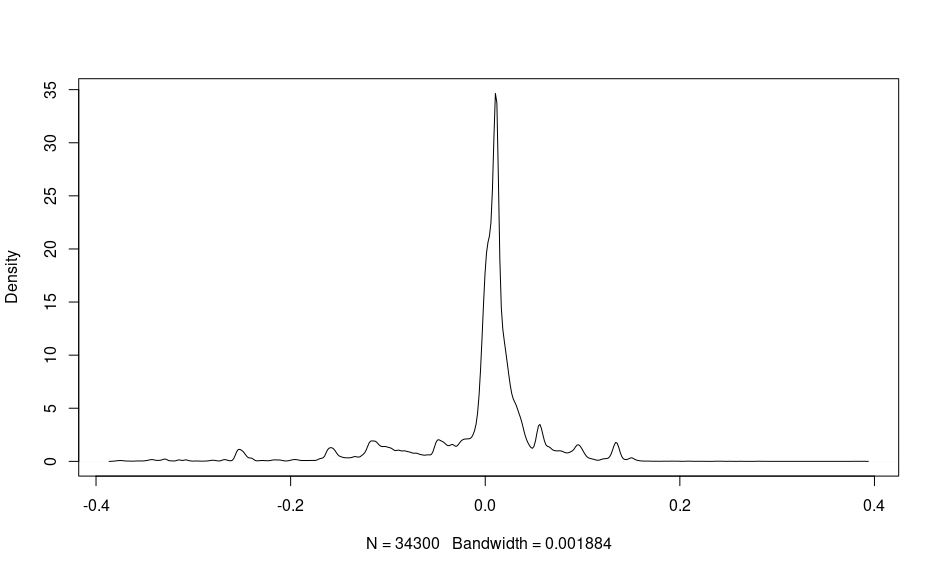
\includegraphics[width=\textwidth]{../local_experiments/io_memory_tests/plots/prediction_density_relative.png}
    \caption{relative errors}
  \end{subfigure}
  \begin{subfigure}[t]{0.49\textwidth}
    \centering
    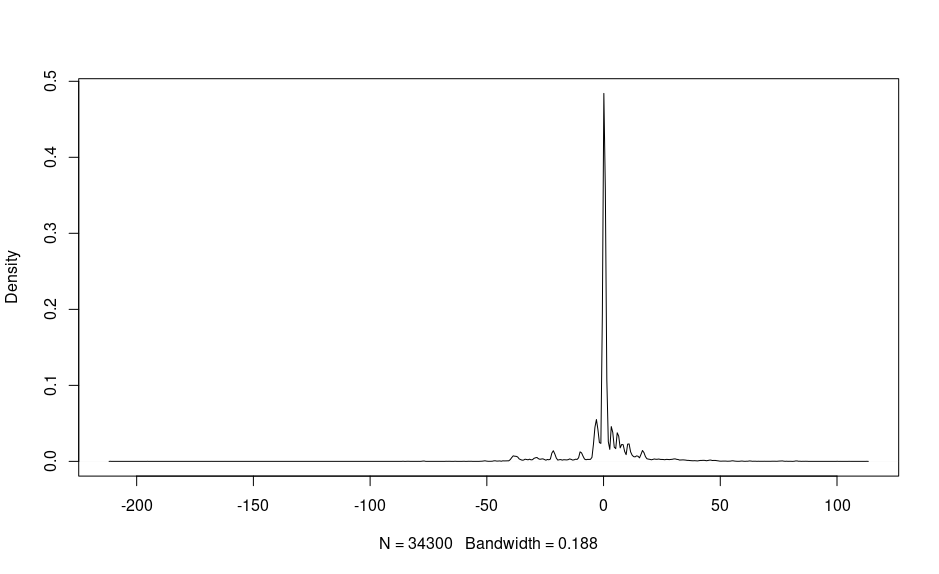
\includegraphics[width=\textwidth]{../local_experiments/io_memory_tests/plots/prediction_density_errors.png}
    \caption{errors (in \si{\mebi\byte})}
  \end{subfigure}
  \caption{Density plots of errors}
  \label{fig:prediction_density}
\end{figure}

\begin{figure}
  \centering
  \begin{subfigure}[t]{\textwidth}
    \centering
    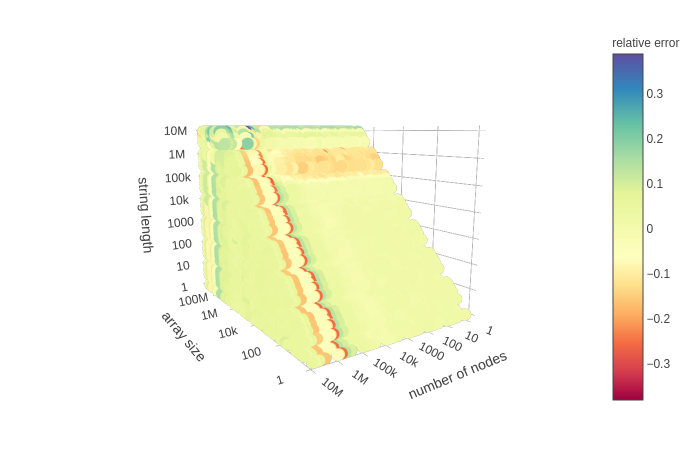
\includegraphics[width=0.5\textwidth]{../local_experiments/io_memory_tests/plots/prediction_relative1.png}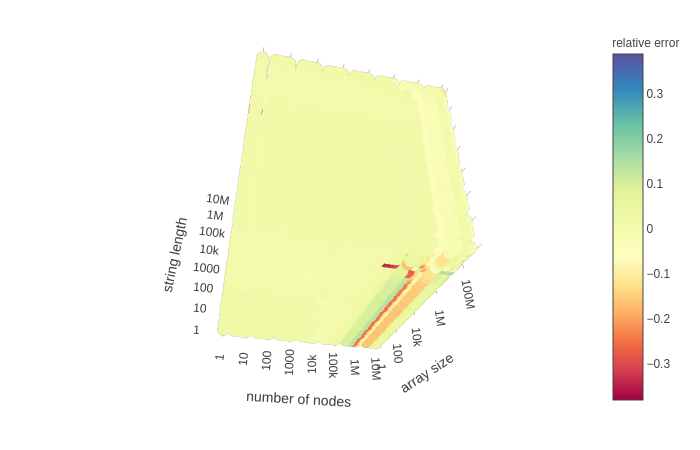
\includegraphics[width=0.5\textwidth]{../local_experiments/io_memory_tests/plots/prediction_relative2.png}
    \caption{relative errors}
  \end{subfigure}
  \begin{subfigure}[t]{0.49\textwidth}
    \centering
    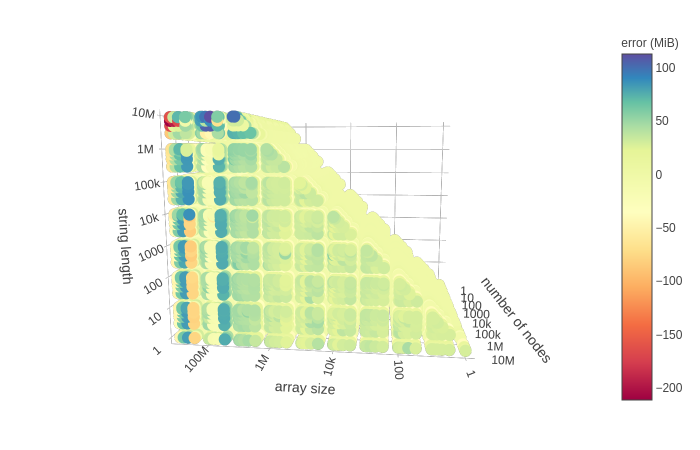
\includegraphics[width=\textwidth]{../local_experiments/io_memory_tests/plots/prediction_errors.png}
    \caption{errors}
    \label{fig:prediction_error_b}
  \end{subfigure}
  \begin{subfigure}[t]{0.49\textwidth}
    \centering
    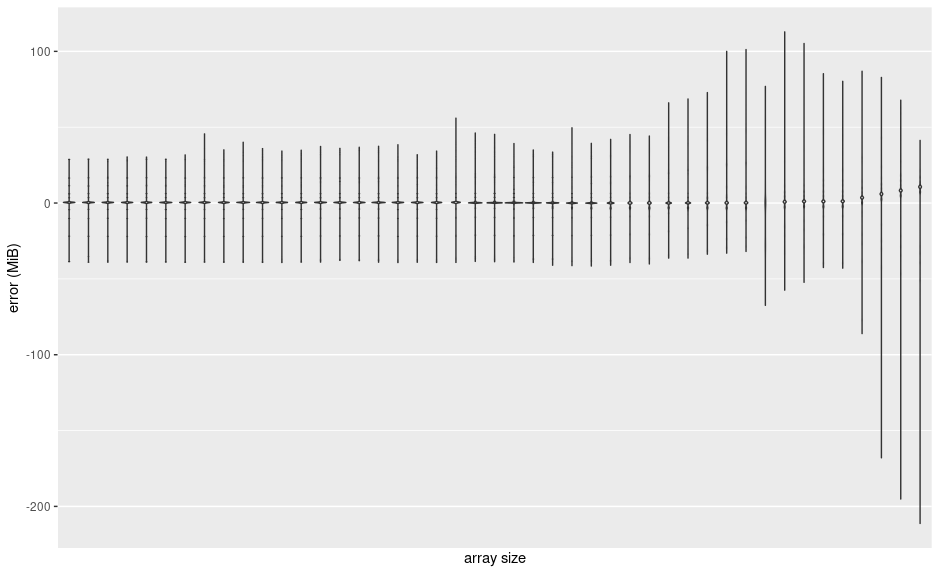
\includegraphics[width=\textwidth]{../local_experiments/io_memory_tests/plots/prediction_violin_array_size.png}
    \caption{errors vs. array size}
  \end{subfigure}
  \begin{subfigure}[t]{0.49\textwidth}
    \centering
    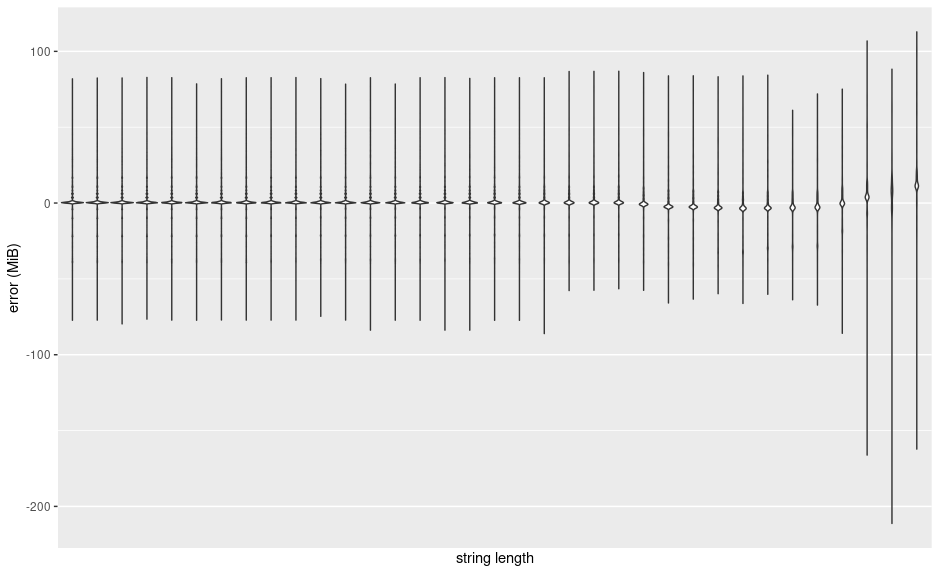
\includegraphics[width=\textwidth]{../local_experiments/io_memory_tests/plots/prediction_violin_string_length.png}
    \caption{errors vs. string length}
    \label{fig:prediction_violin_b}
  \end{subfigure}
  \begin{subfigure}[t]{0.49\textwidth}
    \centering
    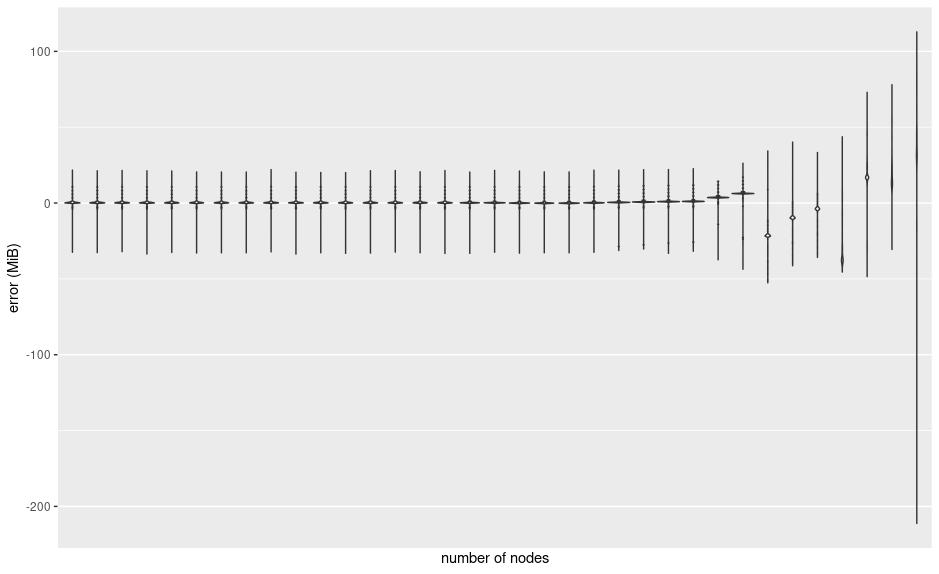
\includegraphics[width=\textwidth]{../local_experiments/io_memory_tests/plots/prediction_violin_num_nodes.png}
    \caption{errors vs. number of nodes}
  \end{subfigure}
  \caption{Prediction errors across all experiments and violin plots of errors
    against the three independent variables}
  \label{fig:predictions}
\end{figure}

\paragraph{Putting the estimates back into action}

We use the estimated memory usage parameters from local experiments to adjust
the application so that it always uses a specified amount of memory. We use a
smaller set of experiments to investigate the resulting application's accuracy.
Namely, \texttt{memoryUsage} is set to $2^0, 2^1, 2^2, \dots,
\SI[exponent-base = 2]{e10}{\mebi\byte}$, while both \texttt{outputSize} and
\texttt{responseSize} are set to any combination of powers-of-two
\si{\mebi\byte} that satisfies total memory usage requirements. With each set of
parameter values, the median of three runs is recorded.

While the errors have more variability, $82\%$ of the relative errors are still
within $\pm10\%$ (see Figure~\ref{fig:posterior_densities}). Unsurprisingly,
highest relative errors occur with low (but not the lowest) expected memory
usage (see Figure~\ref{fig:posterior_errors}). Highest overall errors (both
positive and negative) happen when \texttt{memoryUage} is at its highest,
especially when \texttt{responseSize} is at its highest as well. This again
alludes to the fact that a linear model is not a perfect fit for this situation
and the growth of memory usage experiences non-linear effects with higher
values.

Finally, the violin plots in Figure~\ref{fig:posterior_violins} show that errors
tend to increase with higher \texttt{memoryUsage}. Our linear predictions seem
to perform well with small linked lists, but get significantly less accurate
with higher values of \texttt{responseSize}. Lastly, there is a
positive-to-negative trend in errors with respect to increasing
\texttt{outputSize} that is not captured by our model.

\begin{figure}
  \centering
  \begin{subfigure}[t]{0.49\textwidth}
    \centering
    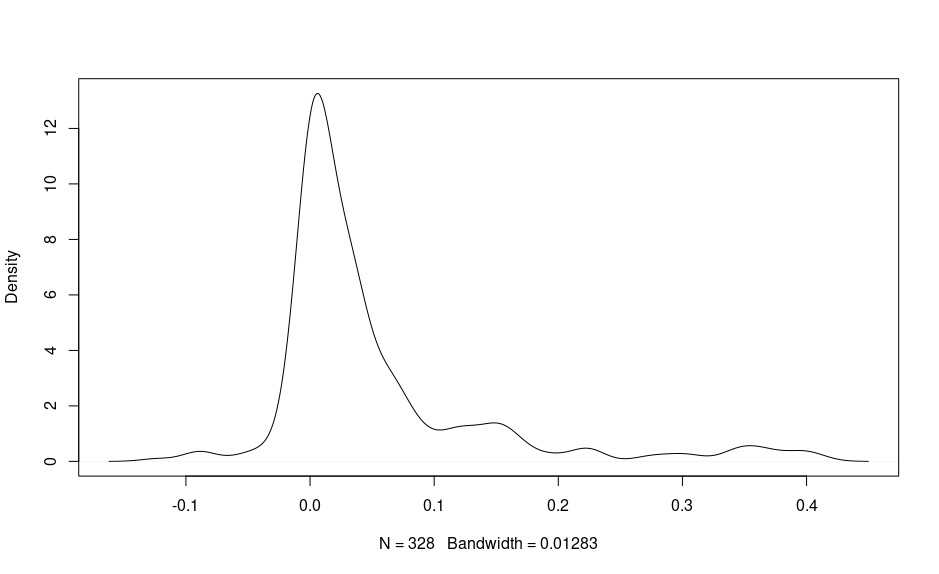
\includegraphics[width=\textwidth]{../local_experiments/io_memory_tests/plots/posterior_density_rel.png}
    \caption{relative errors}
  \end{subfigure}
  \begin{subfigure}[t]{0.49\textwidth}
    \centering
    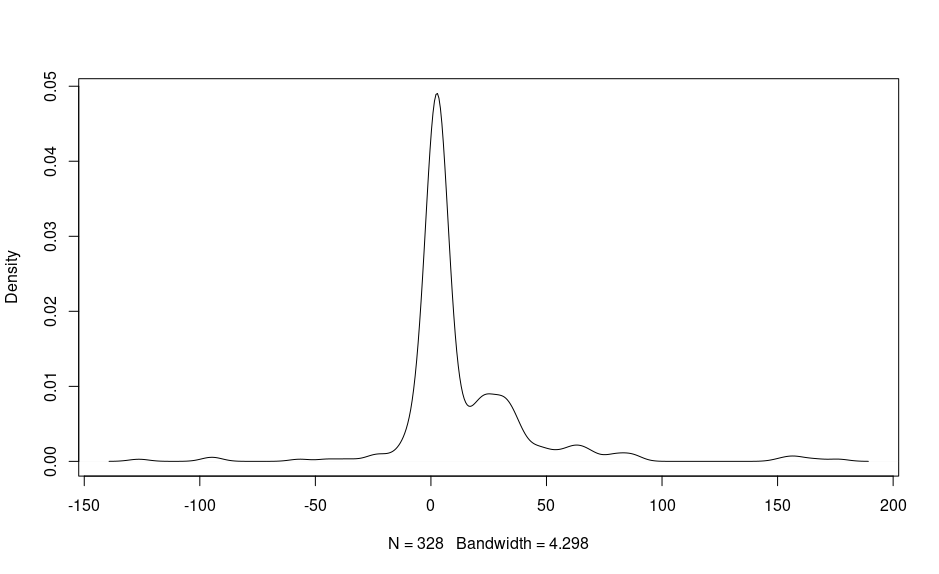
\includegraphics[width=\textwidth]{../local_experiments/io_memory_tests/plots/posterior_density_errors.png}
    \caption{errors (in \si{\mebi\byte})}
  \end{subfigure}
  \caption{Density plots of errors}
  \label{fig:posterior_densities}
\end{figure}

\begin{figure}
  \centering
  \begin{subfigure}[t]{0.49\textwidth}
    \centering
    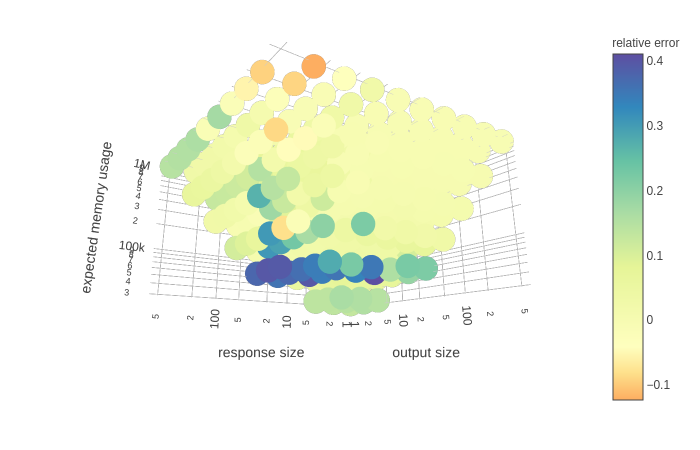
\includegraphics[width=\textwidth]{../local_experiments/io_memory_tests/plots/posterior_relative_errors.png}
    \caption{relative errors}
  \end{subfigure}
  \begin{subfigure}[t]{0.49\textwidth}
    \centering
    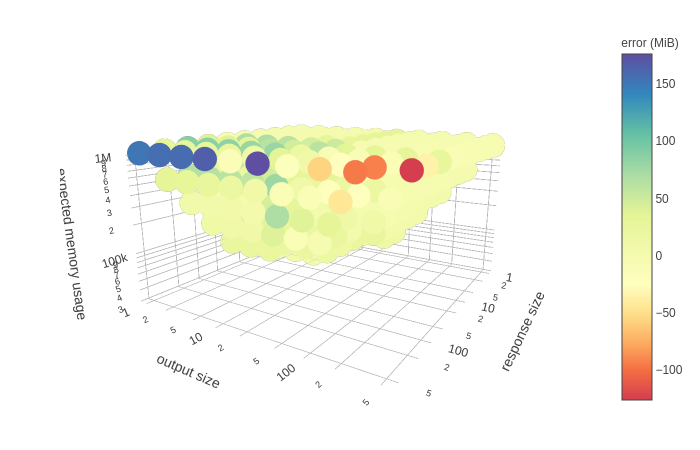
\includegraphics[width=\textwidth]{../local_experiments/io_memory_tests/plots/posterior_errors.png}
    \caption{errors}
  \end{subfigure}
  \caption{Errors in memory usage, comparing the program's measured memory usage
    with the memory usage it was supposed to have}
  \label{fig:posterior_errors}
\end{figure}

\begin{figure}
  \centering
  \begin{subfigure}[t]{0.49\textwidth}
    \centering
    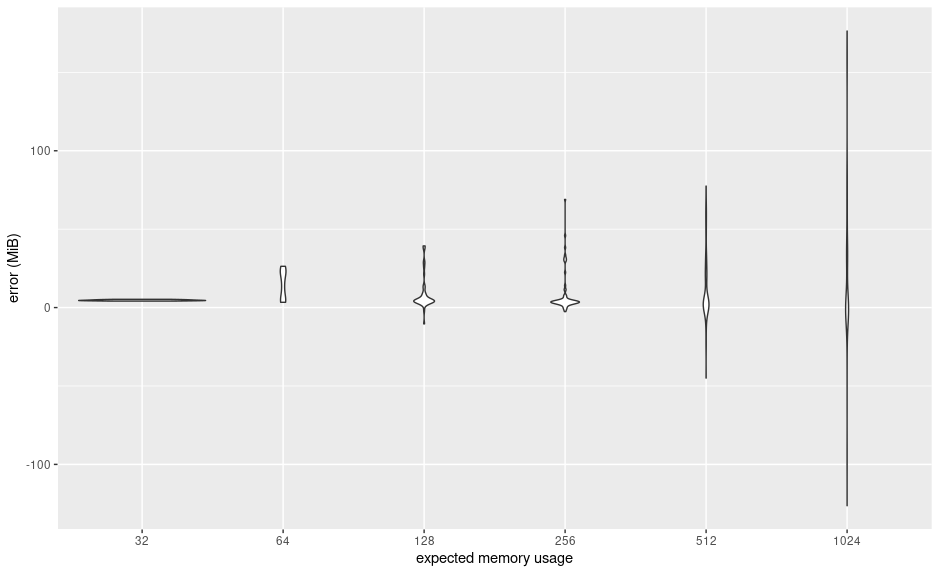
\includegraphics[width=\textwidth]{../local_experiments/io_memory_tests/plots/posterior_error_exp.png}
    \caption{expected memory usage}
    \label{fig:posterior_violin_memory}
  \end{subfigure}
  \begin{subfigure}[t]{0.49\textwidth}
    \centering
    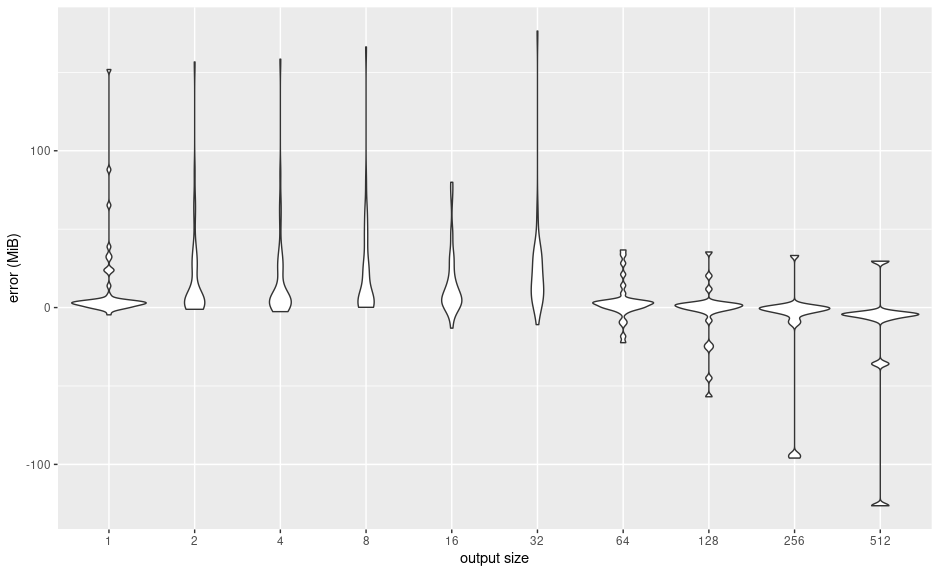
\includegraphics[width=\textwidth]{../local_experiments/io_memory_tests/plots/posterior_error_output.png}
    \caption{output size}
    \label{fig:posterior_violin_output}
  \end{subfigure}
  \begin{subfigure}[t]{0.49\textwidth}
    \centering
    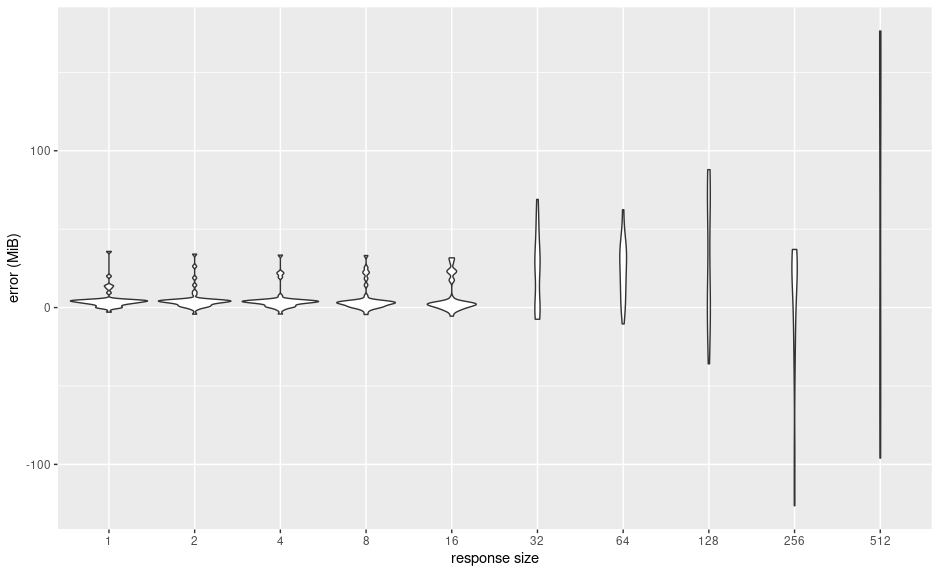
\includegraphics[width=\textwidth]{../local_experiments/io_memory_tests/plots/posterior_error_response.png}
    \caption{response size}
    \label{fig:posterior_violin_response}
  \end{subfigure}
  \caption{Violin plots of errors across independent variables}
  \label{fig:posterior_violins}
\end{figure}

\subsection{Is it taking the right amount of time?}

If Algorithm~\ref{alg:io} is working as intended, total running time of the I/O
simulation process should be
\[
  \texttt{numRequests} \times \left( \texttt{latency} +
  \frac{\texttt{responseSize}}{\texttt{bandwidth}} \right) +
(\texttt{numRequests} - 1) \times \texttt{intervalBetweenRequests}.
\]

As the \texttt{sleep()} routine can be inaccurate for small arguments, we test
a standalone implementation of the algorithm by recording its running time from
within the program itself. We explore all combinations of the following
values\footnote{Combinations of parameters resulting in high (above
  \SI{1}{\minute}) expected running time were discarded in order to make the
  experimental process feasibly efficient.}:
\begin{align*}
  \texttt{numRequests} &= 1, 2, 4, 8; \\
  \texttt{responseSize} &= 0.001, 0.01, 0.1, 1, 10, 100, \SI{1000}{\mebi\byte}; \\
  \texttt{latency} &= 0, 100, \SI{1000}{\milli\second}; \\
  \texttt{bandwidth} &= 0.001, 0.01, 0.1, 1, 10, 100, \SI[per-mode=symbol]{1000}{\mebi\bit\per\second}; \\
  \texttt{intervalBetweenRequests} &= 0, 100, \SI{1000}{\milli\second}.
\end{align*}

Errors above \SI{1}{\second} only occurred with $\texttt{responseSize} =
\texttt{bandwidth} = 1000$, i.e., when constructing a big linked list (with
$\sim \SI{17}{\million}$ nodes) with minimal \texttt{sleep()} breaks during the
construction. In this case, the linked list construction itself takes more
time than the entire process is supposed to take, with errors ranging from
\SI{0.8}{\second} to \SI{9.7}{\second}. All other errors were within
\SI{0.5}{\second} and most of them even within \SI{0.002}{\second}. As
simulating slow memory buildup becomes less relevant when considering transfer
speeds of around \SI[per-mode=symbol]{1}{\gibi\bit\per\second} or more, we
conclude that the algorithm is sufficiently accurate.

\section{Generating Various Usage Patterns} \label{sec:usage_patterns}

Hitherto the simulated user of the application was restricted to sending one or
more messages at regular intervals. However, real usage patterns are often more
complicated than that. For instance, a website might have more users during the
day than at night, it might be slowly becoming more popular, and it might
experience a spike in the number of users during an important event. In this
section we present an approach that can simulate usage (or workload) patterns
represented by any computable function.

Recall that a periodic workload is defined by the three parameters
\texttt{experimentDuration}, \texttt{batchesPerSecond}, and
\texttt{messagesPerBatch}. We define a `functional' workload as a 4-tuple
consisting of a \texttt{function} string and three floating-point numbers:
\texttt{binWidth}, \texttt{initialX}, and \texttt{finalX}. The \texttt{function}
variable contains a function of a single variable $x$ expressed in JavaScript
syntax. For example, in order to represent
\begin{equation} \label{eq:example_function}
  f(x) = 10 + x + 5\sin(-4x + 4) + 10\exp \left( -\frac{(x - 10)^2}{2} \right),
\end{equation}
we would construct the following \texttt{function} string:
\begin{lstlisting}[language=JavaScript]
10 + x + 5 * Math.sin(-4 * x + 4) + 10 * Math.exp(-Math.pow(x - 10, 2) / 2).
\end{lstlisting}
Variables \texttt{initialX} and \texttt{finalX} define the interval of $x$
values we want to simulate. Finally, \texttt{binWidth} is the discretisation
parameter. In order to simulate the behaviour of a continuous function, we need
to sample its values at different values of $x$, and \texttt{binWidth} defines
the distance between different samples (see
Figure~\ref{fig:functional_workload}).

The \texttt{function} defines the workload frequency, while $x$ is the time
variable. The number of messages we are supposed to send in an interval of size
\texttt{binWidth} is then \texttt{binWidth} multiplied by the \texttt{function}
evaluated at some point within the interval (in this case we choose the middle
of the interval). We evaluate the \texttt{function} by replacing all occurrences
of $x$ with the value of $x$ that corresponds to the interval of
interest\footnote{We only replace occurrences of $x$ that are not part of a
  longer word. This is needed so that the \texttt{x} in \texttt{exp} is not
  replaced.} and sending the resulting string to a JavaScript evaluation engine
(since Java itself has no evaluation function of its own). We then send the
computed number of messages and wait \texttt{binWidth} time before evaluating
the \texttt{function} at the next interval.

The implementation assumes that $x$ (along with \texttt{binWidth}) is measured
in seconds, and the \texttt{function} is measured in \si{\hertz}. It is also
important to set up the \texttt{binWidth} parameter so that the number of
requests we send at a time is higher than zero, but also not too
high---otherwise the simulation becomes inaccurate.

\begin{figure}
  \centering
  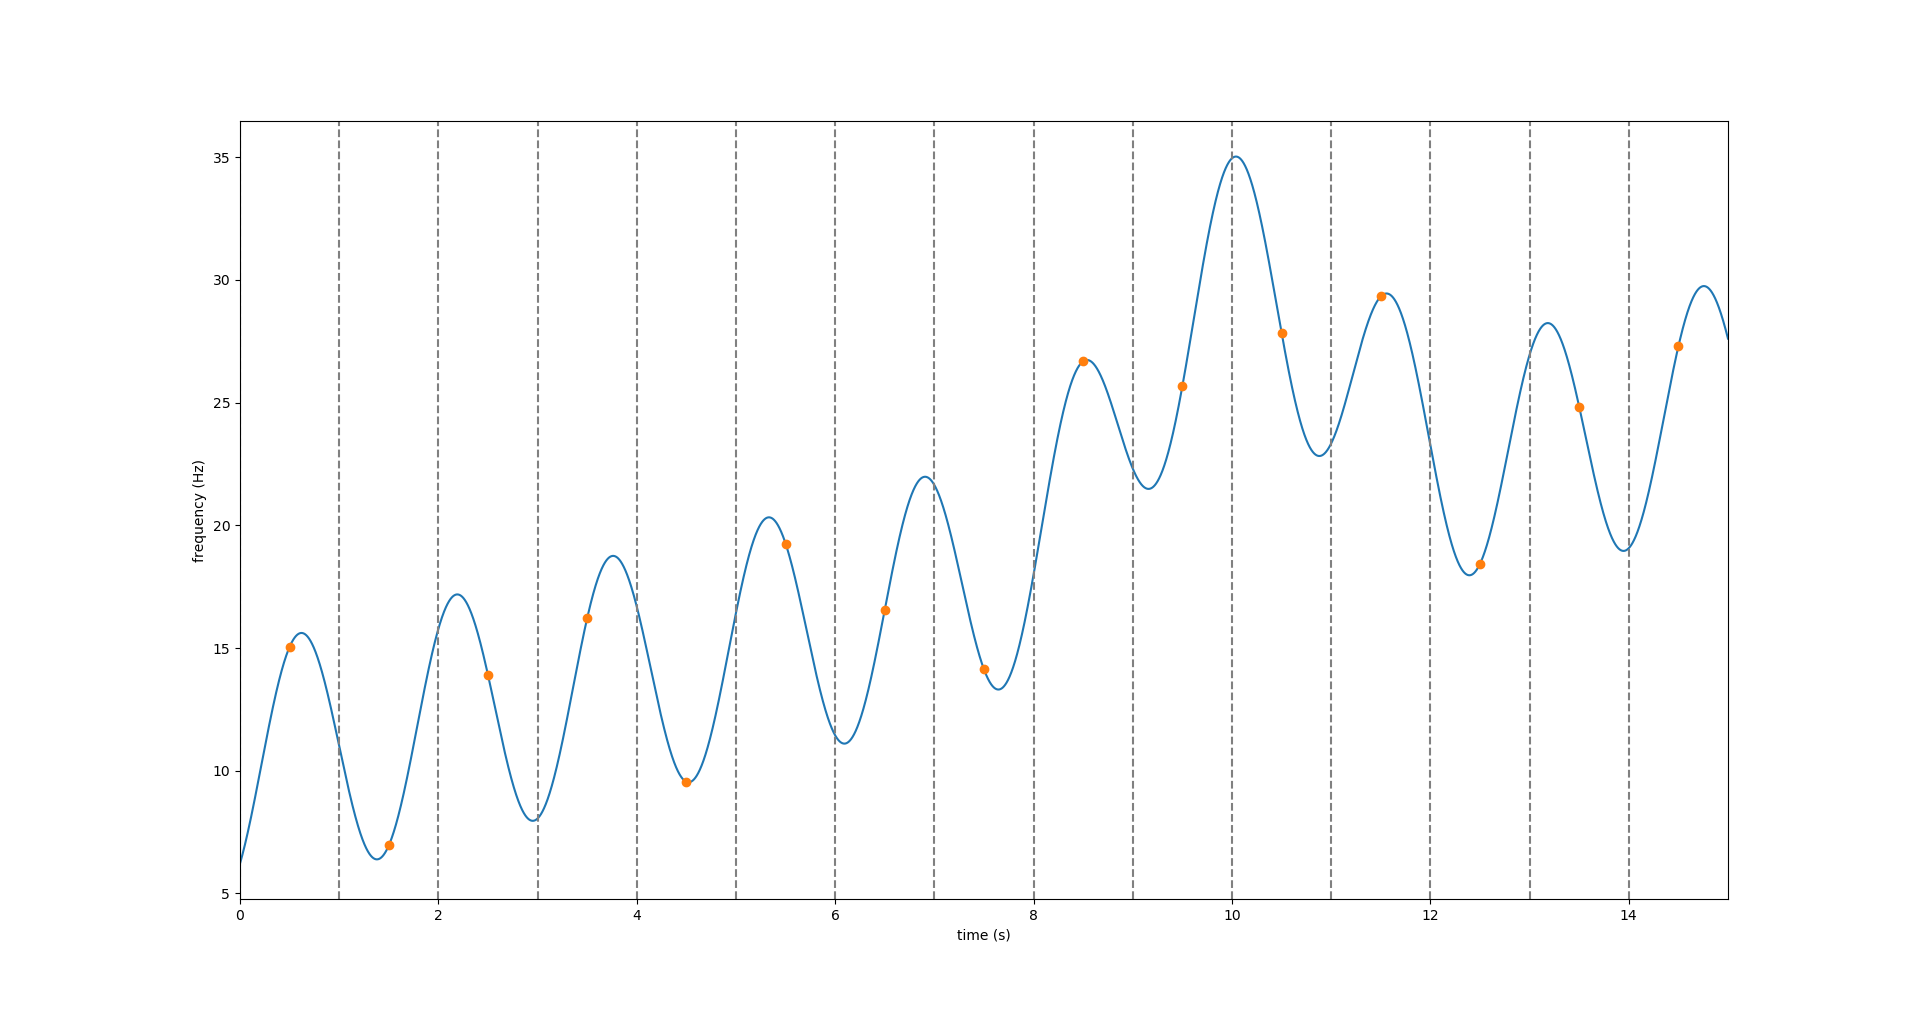
\includegraphics[width=\textwidth]{../plots/functional_workload.png}
  \caption{Function~\eqref{eq:example_function} plotted between $x=0$ and
    $x=15$ with intervals of \texttt{binWidth} marked by dashed vertical lines
    and the function's values at their centres marked by yellow dots}
  \label{fig:functional_workload}
\end{figure}

\section{Validation} \label{sec:validation}

In this section we tackle the question: does the experimental data match our
expectations? We have expectations for both memory and CPU usage. For memory,
the parameter \texttt{memoryUsage} defines our expectation for how much memory
should be used during the experiment (per component, that is). For CPU, we can
measure how long one component takes to handle a single message and compare this
data sample with \texttt{cpuTime}.

In both cases, we answer the question by fitting a probability distribution to
the data and calculating the \emph{$p$-value} of the expectation, i.e., the
probability that a value generated by the fitted probability distribution is at
least as far away from the mode\footnote{We use modes instead of means for two
  reasons:
  \begin{itemize*}
  \item the mode represents a more reasonable best guess for our expectation
    (which is not an actual expected value of the distribution or the data!),
  \item the distribution used for the CPU data could have an infinite mean for
    some values of its parameters.
  \end{itemize*}} as our original expectation (see Figure~\ref{fig:p_value} for
an example). Note that in order for the fitted distribution to be realistic, we
recommend running about twenty experiments for each configuration of parameters.

\begin{figure}
  \centering
  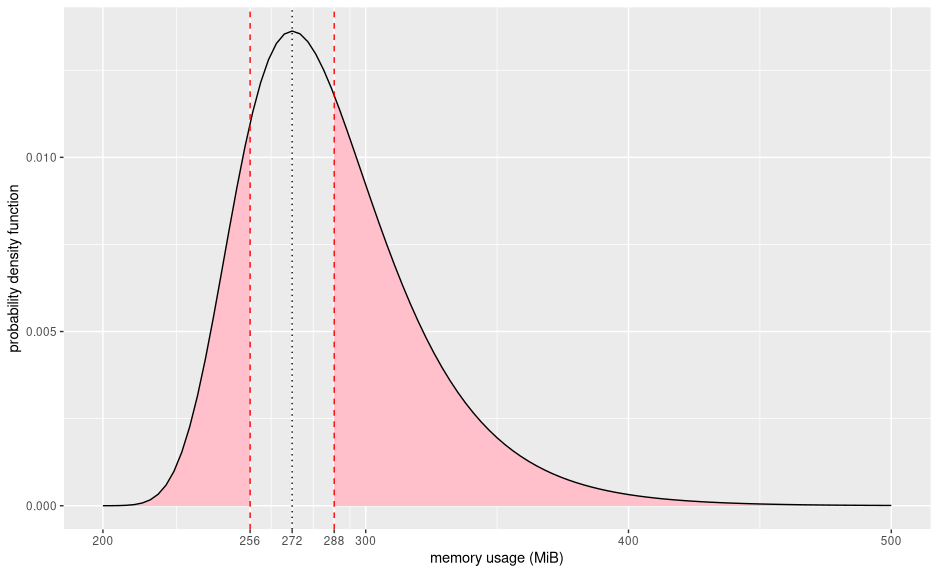
\includegraphics[width=\textwidth]{../plots/p_value.png}
  \caption{The visualisation of the $p$-value for memory usage data with
    \texttt{memoryUsage} set to \SI{256}{\mebi\byte}. The $p$-value is
    calculated by integrating the shaded area under the probability density
    function. The black dotted line marks the mode of the fitted probability
    distribution. The first dashed red line shows our expected value of memory
    usage, while the second such red line is symmetric to the first one with
    respect to the mode of the distribution.}
  \label{fig:p_value}
\end{figure}

\subsection{Memory}

Each experiment gives us a time series of memory usage values over time. We
reduce each series to a single value by taking its maximum value, as lower
values represent either memory usage before all variables are initialised or
memory usage after some variables have already been claimed by the garbage
collector. This collection of maximum values then follows Gumbel distribution,
which is meant to represent any maximum values \cite{gumbel1935valeurs}. We fit
this distribution to the data using the R package \texttt{ismev}
\cite{heffernan2012ismev} and calculate the $p$-values as previously described.

The results are summarised in Table~\ref{tbl:gumbel}. If we make an arbitrary
decision to consider data as in line with our expectations if the $p$-value is
greater than 0.05, then all four data sets pass this test. However, the
$p$-value clearly shows that the \SI{64}{\mebi\byte} experiment barely passes,
while the 128 and \SI{512}{\mebi\byte} experiments match our expectations
extremely well!

The near-failure of the \SI{64}{\mebi\byte} test can be partially explained by
the fact that---unlike all other data sets---this one has no data points below
the expected amount of memory usage (i.e., all measurements are above
\SI{70}{\mebi\byte}). This skews the data too far to the right. More generally,
the goodness-of-fit plots in Figure~\ref{fig:gumbel_fit} show a reasonable fit
for all except perhaps the \SI{128}{\mebi\byte} data set.

\begin{table}
  \centering
  \caption{Expected memory usage compared to the mode of the fitted distribution}
  \begin{tabular}{c c c c}
    \toprule
    Our expectation (\si{\mebi\byte}) & Mode (\si{\mebi\byte}) & $p$-value \\
    \midrule
    \tablenum{64} & \tablenum{77.1} & \tablenum{0.056} \\
    \tablenum{128} & \tablenum{128.1} & \tablenum{0.998} \\
    \tablenum{256} & \tablenum{272.3} & \tablenum{0.583} \\
    \tablenum{512} & \tablenum{514.9} & \tablenum{0.983} \\
    \bottomrule
  \end{tabular}
  \label{tbl:gumbel}
\end{table}

\begin{figure}
  \centering
  \begin{subfigure}[t]{0.49\textwidth}
    \centering
    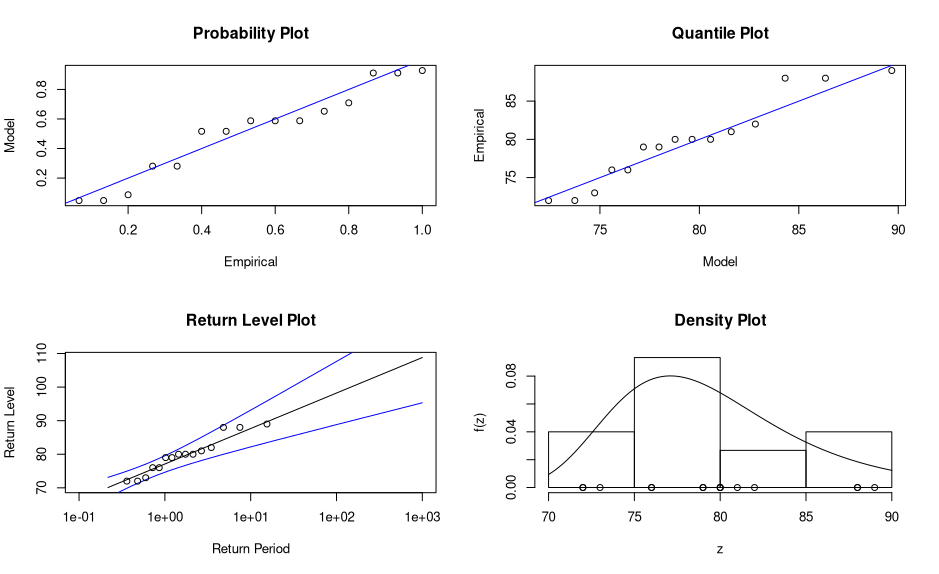
\includegraphics[width=\textwidth]{../plots/memory_fit_64.png}
    \caption{expected memory usage: \SI{64}{\mebi\byte}}
  \end{subfigure}
  \begin{subfigure}[t]{0.49\textwidth}
    \centering
    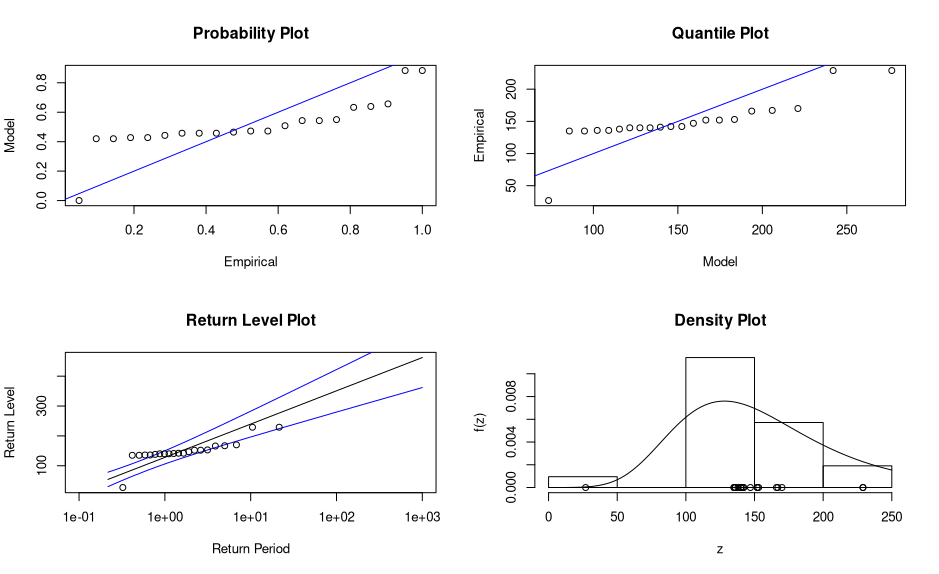
\includegraphics[width=\textwidth]{../plots/memory_fit_128.png}
    \caption{expected memory usage: \SI{128}{\mebi\byte}}
  \end{subfigure}
  \begin{subfigure}[t]{0.49\textwidth}
    \centering
    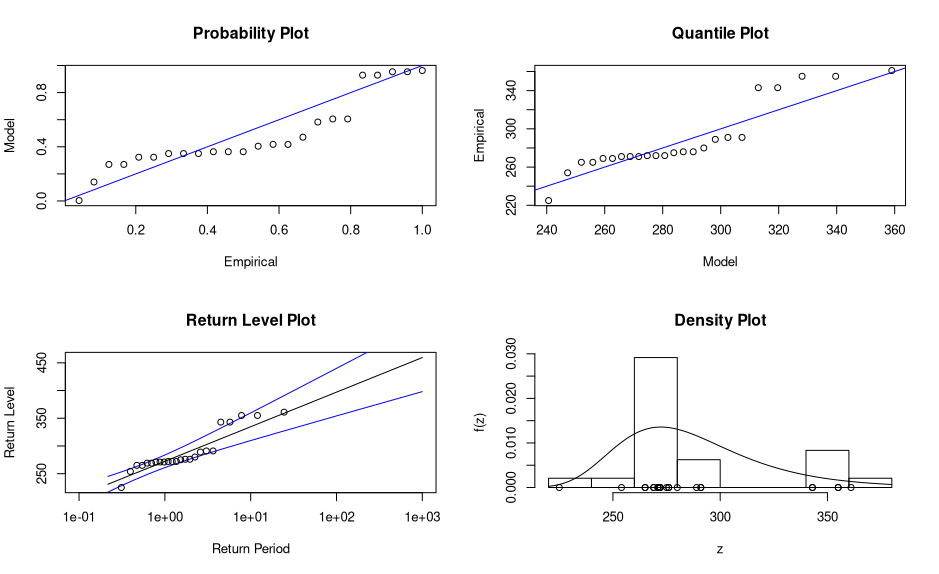
\includegraphics[width=\textwidth]{../plots/memory_fit_256.png}
    \caption{expected memory usage: \SI{256}{\mebi\byte}}
  \end{subfigure}
  \begin{subfigure}[t]{0.49\textwidth}
    \centering
    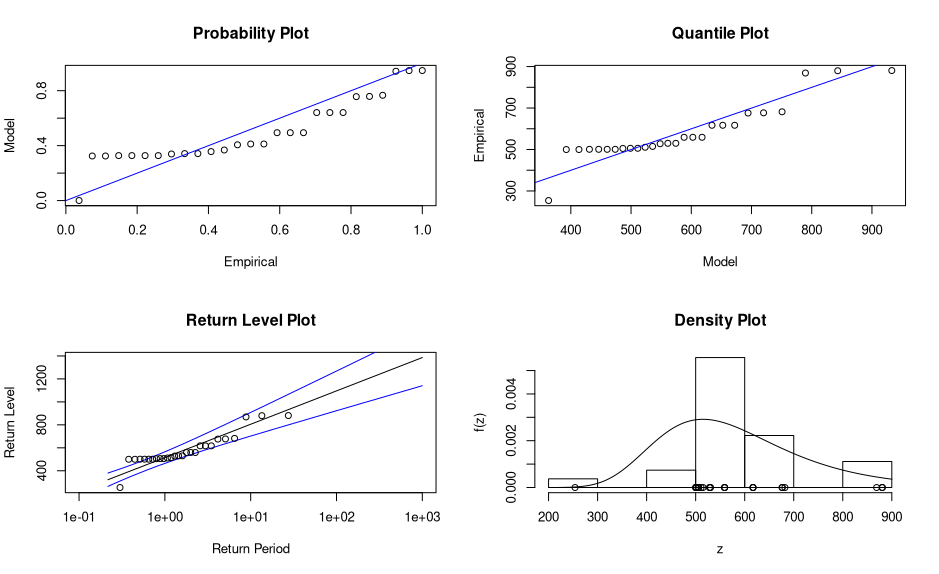
\includegraphics[width=\textwidth]{../plots/memory_fit_512.png}
    \caption{expected memory usage: \SI{512}{\mebi\byte}}
  \end{subfigure}
  \caption{Goodness-of-fit plots for four different values of expected memory
    usage based on our experiments from Section~\ref{sec:experiments}}
  \label{fig:gumbel_fit}
\end{figure}

\subsection{CPU Time}

While we have CPU data expressed as a set of time series with values ranging
between zero and one, our only CPU-based expectation is that of time, i.e., the
amount of time it takes for one component to handle a single message. We can
transform out data into this form by reducing each time series to the difference
in time between first and last data points.

Without a solid statistical argument, we try fitting two asymmetric heavy-tailed
distributions: log-normal and Fr\'{e}chet. We are using a single data set with
\texttt{cpuTime} set to zero. The plots in Figure~\ref{fig:frechet_fit} clearly
show that the Fr\'{e}chet distribution provides a much better fit than the
log-normal distribution.

The mode of the Fr\'{e}chet distribution with shape $\alpha$, scale $s$, and
location $m$ can be calculated as
\[
  M = m + s \left( \frac{\alpha}{1 + \alpha} \right)^{1/\alpha},
\]
which with our data becomes $M = 6.1$. Recall that the expected amount of CPU
time for this experiment is \SI{0}{\second}. Comparing it to the fitted
distribution gives a $p$-value of 0.246---a value good enough to be accepted yet
showing significant uncertainty stemming from the ambitious goal of having
everything run in zero time.

\begin{figure}
  \centering
  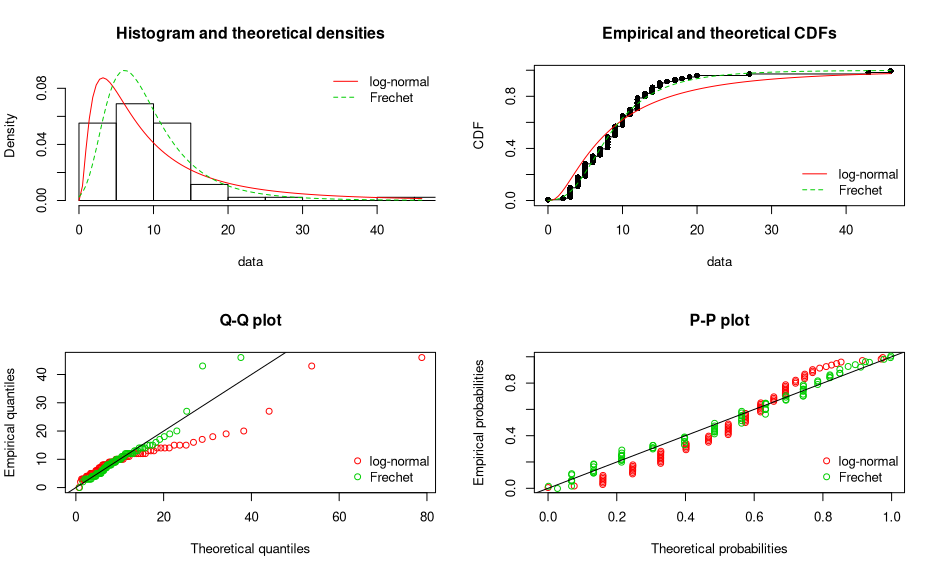
\includegraphics[width=\textwidth]{../plots/cpu_time_distributions.png}
  \caption{Evaluation of how well the log-normal and Fr\'{e}chet distributions fit
    the data using four standard plots}
  \label{fig:frechet_fit}
\end{figure}


\section{Conclusions and Future Work} \label{sec:conclusions}

We conclude with an overview of possible directions for future work, examining
the weaknesses of our work as it is and considering ways to improve it.

%\paragraph{Compatibility with OpenShift}
%connections between services on OpenShift (special case: Prometheus and
%TaskManager), not properly tested.
% TODO: cover what needs to be done regarding OpenShift

\paragraph{End-to-end latency}
Another performance metric that could be useful and interesting to look at is
the latency of the entire system, measured from the moment the control server
sends its message, to the output of the last component being returned to the
same server. With the current implementation, there are two issues regarding the
implementation of this metric:
\begin{itemize}
\item With the DAG support, there is no last component: a graph can
  have any number of nodes with no out-links. Perhaps there could be an
  additional parameter for each component that determines whether we are
  interested in its output. The union of the `interesting' outputs could be
  transmitted back to the server.
\item Prometheus would have to collect information from the control server
  itself. This means that the control server would have to concurrently run an
  additional server in order to respond to requests by Prometheus. It might be
  better in the long run to reimplement the control server using a platform with
  native support for Prometheus, e.g., RabbitMQ.
\end{itemize}

\paragraph{Higher memory usage capabilities}
Currently, memory usage (as implemented using an array of bytes) is limited to
about \SI{2}{\gibi\byte}, and similar restrictions apply to the memory usage of
I/O operations as well. Higher numbers can be supported by replacing the array
and the linked list with an array of arrays and an array of linked lists,
respectively. This feature was not implemented simply because it is more
important to make sure that the product is working correctly and can be useful
than it is to scale it to higher numbers, and this feature would add unnecessary
complexity to core parts of the system.

\paragraph{Topologies with cycles}
We demonstrated how components can be arranged as any directed \emph{acyclic}
graph, but what about cycles? Perhaps we want a message to travel around a
cycle a few times, or maybe even an unbounded amount of times until the experiment
terminates. As Apache Flink supports cyclic topologies (as long as the output is
different with each iteration)
\cite{stackoverflow,DBLP:journals/pvldb/EwenTKM12}, this could be a valuable
direction for further work.

\paragraph{Convenience}
The system in its current state is a collection of tools and scripts, where one
often needs to make changes to the Makefile and/or Python/R scripts in order to
make the system do the right thing. Little development effort has gone into
integrating different parts of the system for two reasons:
\begin{itemize}
\item OpenShift can act like a stubborn child and require several semi-manual
  attempts in order to get it to behave as expected.
\item At this point in the development, it is not entirely clear what the
  primary use cases of the system are. The way the system is used for testing
  might not reflect some of the desired use cases.
\end{itemize*}

\paragraph{Memory usage during I/O simulation}
With the current implementation, each `file' `downloaded' during an I/O
simulation is immediately marked for garbage collection. Alternatively, the
`downloaded' data could be kept for a longer period of time, i.e.,
\begin{itemize}
\item if the I/O mode is set to \texttt{startup}, data structures constructed
  during I/O simulation could be kept for the entire execution of the program;
\item if the I/O mode is set to \texttt{regular}, the data could be kept until
  the component finishes processing the message.
\end{itemize}
While both alternatives represent realistic real-life scenarios, keeping the
data for longer would make memory usage more predictable. Perhaps both options
could be implemented.

\paragraph{Resource constraints}
The initial goal of this project was to investigate how a variety of distributed
applications behave under different resource constraints. So far, no constraints
have been mentioned.

On OpenShift, one can set CPU and memory constraints in several ways. First,
each constraint can be declared either for a specific pod, or for the sum total
of all pods. Second, we can either declare \emph{limits} or \emph{requests},
i.e., upper or lower bounds respectively. Perhaps it would be most appropriate
for our needs to set requests equal to limits, declaring them separately for
each pod.

CPU resources are measured in \emph{millicores}. For example, setting a CPU
limit of 1500~millicores corresponds to allowing the application to use up
to one and a half processor cores. This restriction can affect running time and
thus can be analysed using the statistical methods developed for
\texttt{cpuTime}.

The situation with memory resource control is less optimistic. While we get to
restrict total memory usage using familiar units of \si{\mebi\byte} and
\si{\gibi\byte}, if the application tries to use more than the allocated amount
of memory, it gets terminated by OpenShift. Hence memory usage can be measured
but not controlled.

\bibliographystyle{abbrv}
\bibliography{report}
\end{document}